% !TeX root = ../dokumentation.tex

\addchap{\langanhang}

\iflang{de}{
    \begin{enumerate}[label=\Alph*.]
        \item Datenquellen
        \item Übersicht: Wahlprogramme
        \item Training
              % \item Tabellen
    \end{enumerate}
}

\pagebreak

\setcounter{section}{0}
\renewcommand{\thesection}{\Alph{section}}
\counterwithin{figure}{section}
\counterwithin{table}{section}
\counterwithin{example}{section}

%\includepdf[pages=-,scale=.9,pagecommand={}]{Aufgabenstellung.pdf} % PDF um 10% verkleinert einbinden --> Kopf- und Fußzeile  werden so korrekt dargestellt. Die Option `pages' ermöglicht es, eine bestimmte Sequenz von Seiten (z.B. 2-10 oder `-' für alle Seiten) auszuwählen.
%\pagebreak

\section{Datenquellen} \label{ch:dataAppendix}

\subsection*{Tweets}

\begin{example}[H]
    \begin{subexample}{0.45\textwidth}
        \small
        Kritischer Austausch bei der Diskussion @co2abgabe. Der CO2-Preis im \#Emissionshandel steigt, das Vertrauen in dieses Instrument muss weiter wachsen! https://t.co/hv1VFPBJrv
        \caption{Beispieltweet von \textit{\_martinneumann}}
    \end{subexample}\hfill
    \begin{subexample}{0.45\textwidth}
        \small
        Treten Sie zurück, Herr Reul! Bin fassungslos, mit welcher Selbstherrlichkeit die NRW-Landesregierung die Profitinteressen von RWE im \#HambacherForst durchsetzt. Der heutige Polizeieinsatz gegen friedliche Sitzblockierer war brutal, selbst Journalisten sind geschlagen worden(1/3) https://t.co/0A3JbnUMmV
        \caption{Beispieltweet von \textit{zdebelhubertus}}
    \end{subexample}\hfill
    \caption{Beispiel für Tweets von Politikern auf Twitter \autocite{saltzer_finding_2022}} \label{list:exampleTweets}
\end{example}

\subsection*{Wahlprogramme}

\begin{figure}[H]
    \centering
    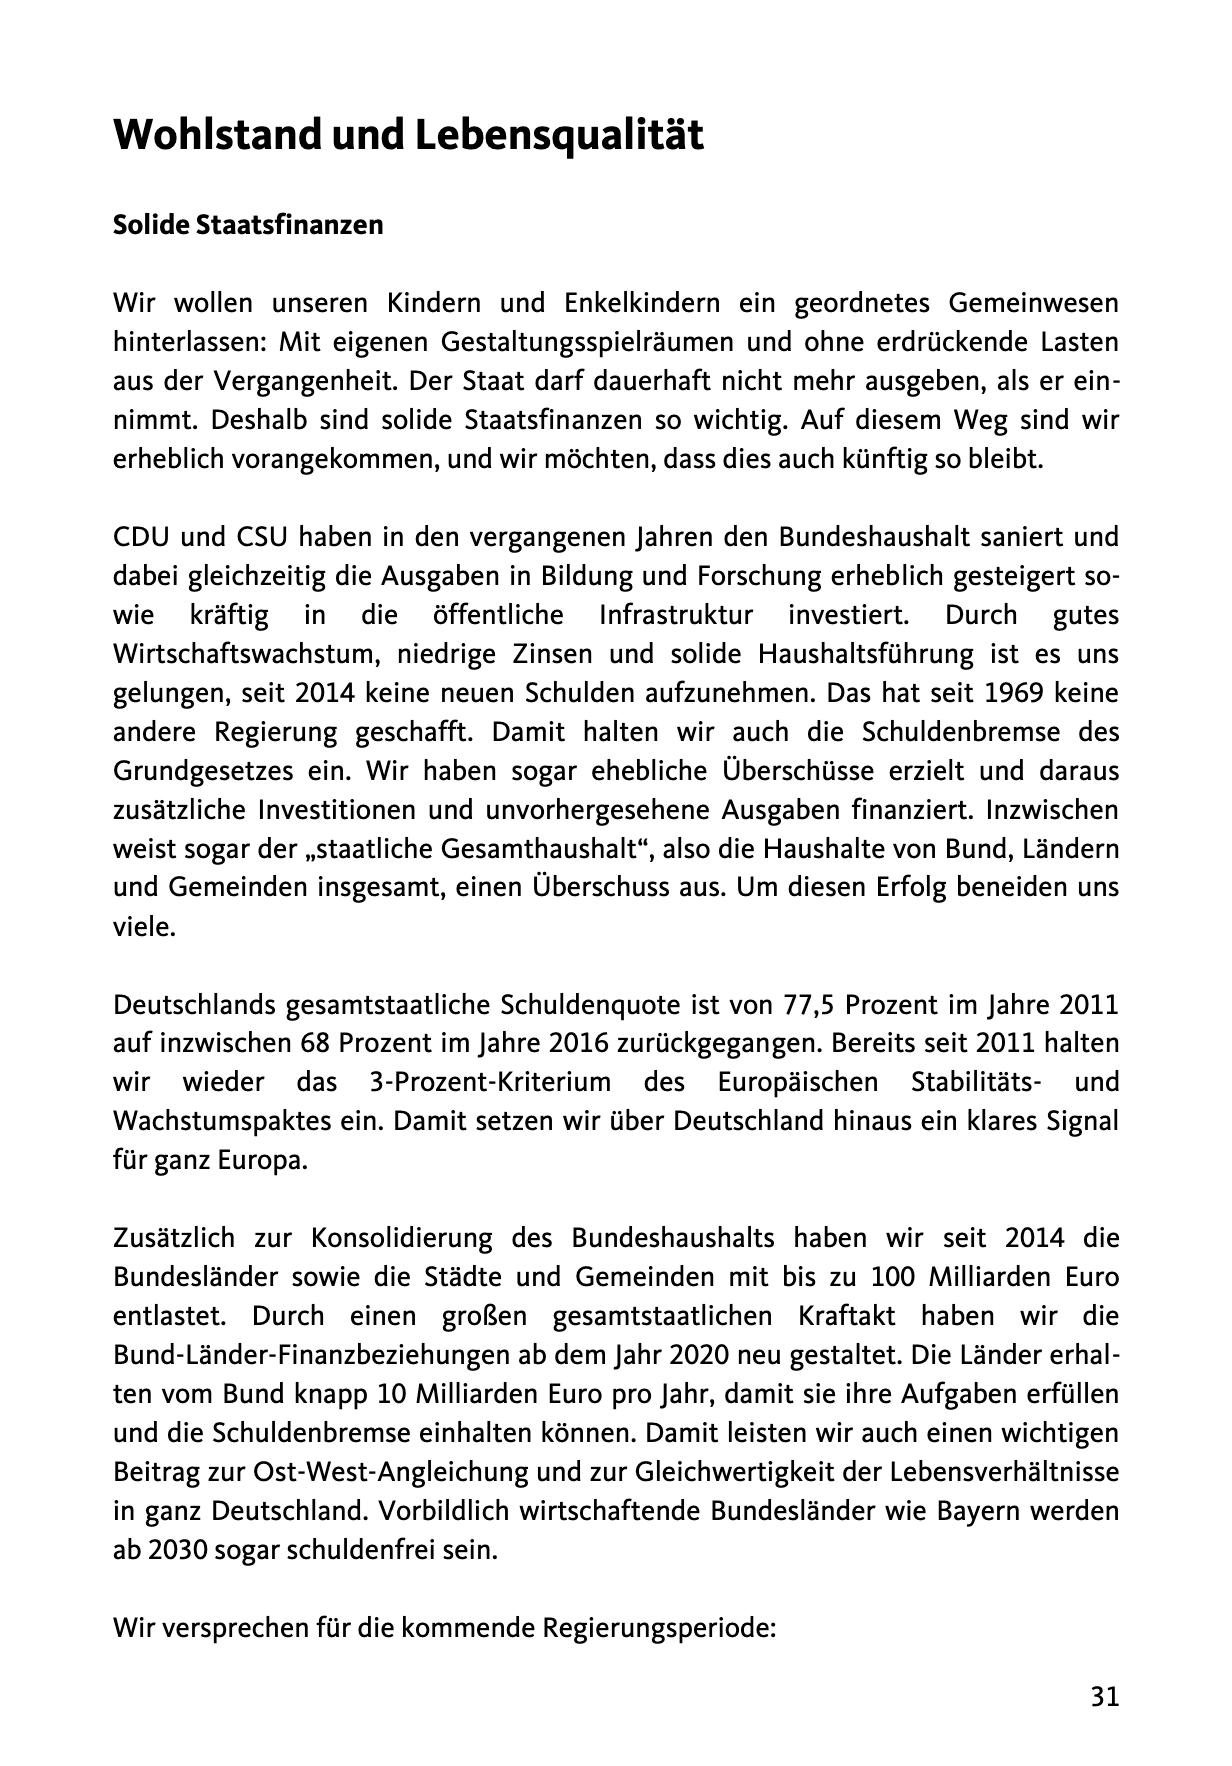
\includegraphics[width=0.9\textwidth]{data/images/appendix/union_btw17_ausschnitt.png}
    \caption{Ausschnitt aus dem \href{https://archiv.cdu.de/system/tdf/media/dokumente/170703regierungsprogramm2017.pdf?file=1}{Wahlprogramm der CDU} zur Bundestagswahl 2017}
    \label{fig:partyProgramExapleCdu}
\end{figure}

\begin{figure}[H]
    \centering
    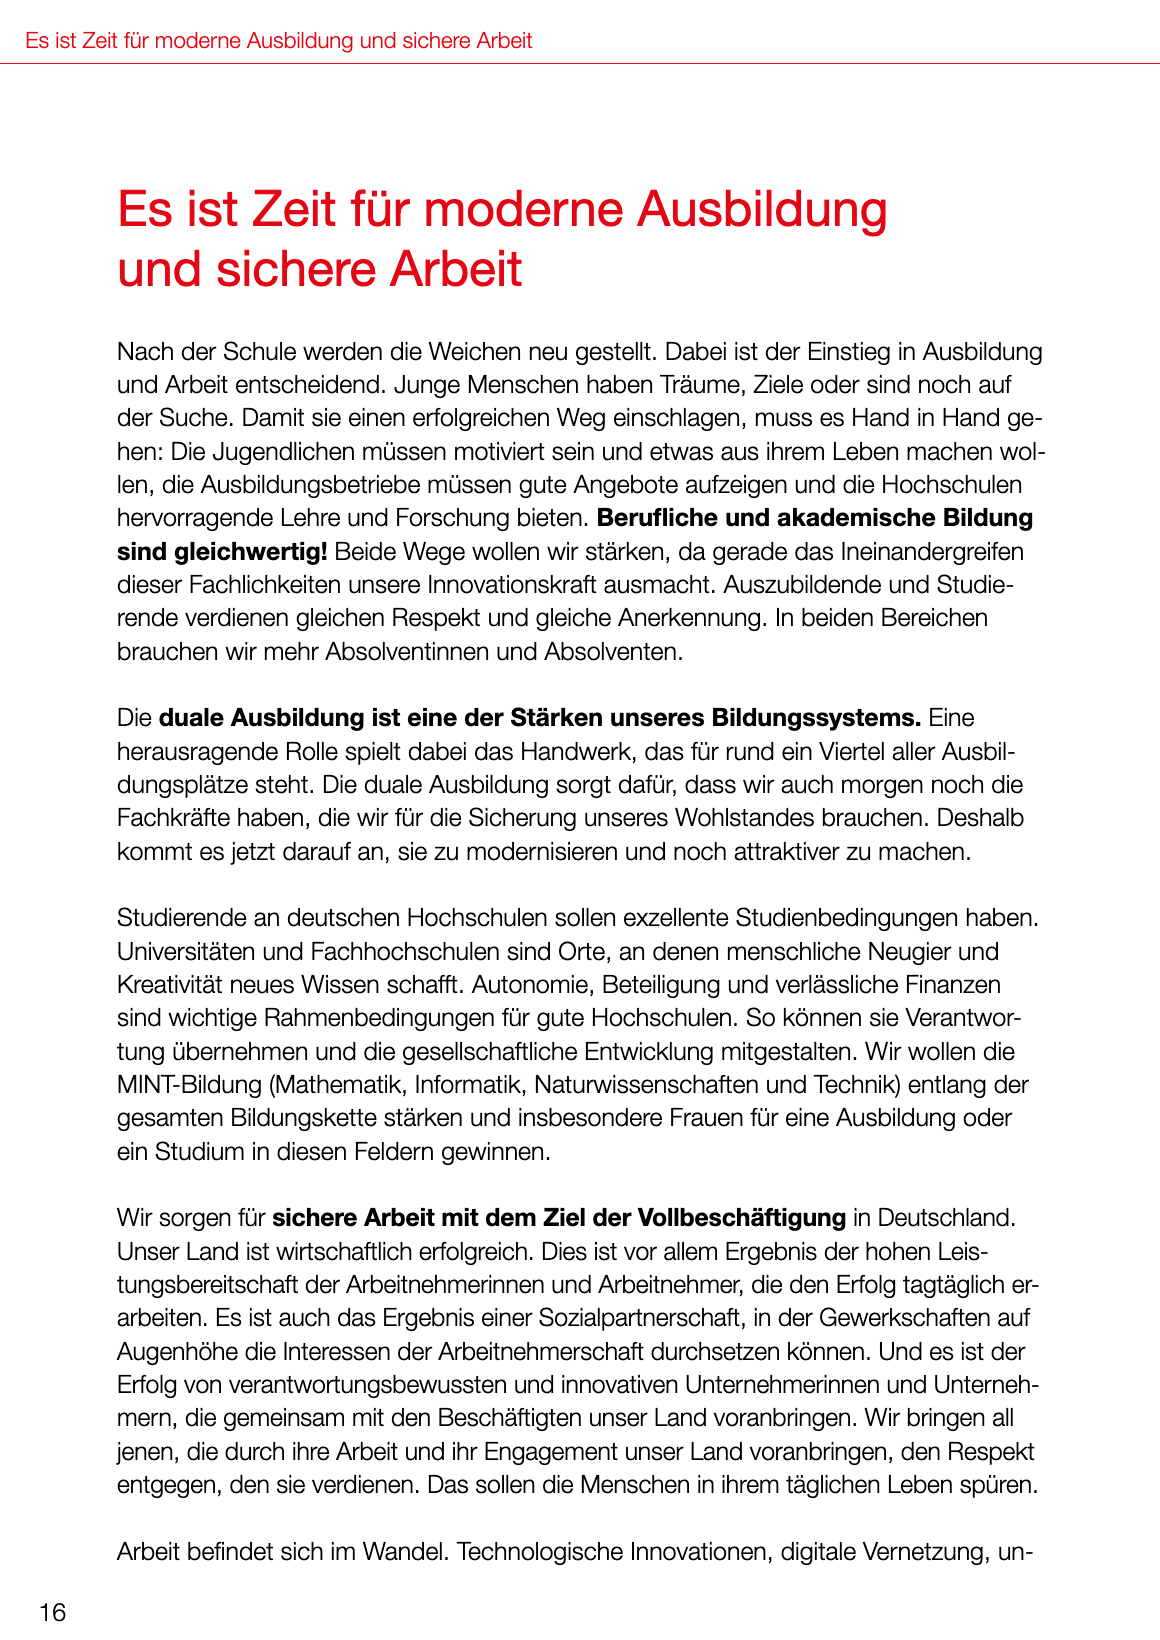
\includegraphics[width=0.9\textwidth]{data/images/appendix/spd_btw17_ausschnitt.png}
    \caption{Ausschnitt aus dem \href{https://www.spd.de/fileadmin/Dokumente/Regierungsprogramm/SPD_Regierungsprogramm_BTW_2017_A5_RZ_WEB.pdf}{ Wahlprogramm der SPD} zur Bundestagswahl 2017}
    \label{fig:partyProgramExapleSpd}
\end{figure}

\subsection*{Reden}

\begin{example}[H]
    Sehr geehrter Herr Präsident! Liebe Kolleginnen und Kollegen! Man kann hier im Hohen Haus offenbar nicht oft genug wiederholen: Statt einer emotional geführten Debatte ist eine sachliche, an Fakten orientierte Analyse angemessen und notwendig. Dazu gehören zwei Grunderkenntnisse: Wir brauchen kein Rüstungsexportkontrollgesetz und auch kein generelles Verbot des Exports von Rüstungsgütern.

    (\{0\})

    Wir haben folgende Interessen: Erstens, nationale Verteidigungsfähigkeit. Zentrale Aufgabe eines Staates ist die Gewährleistung der Sicherheit seiner Bürgerinnen und Bürger, also eine unabhängige Wehr- und Abwehrfähigkeit.

    Zweitens, Erhalt einer eigenen wehrtechnischen Industrie. Wir brauchen eine deutsche Verteidigungs- und wehrtechnische Industrie. Oder wollen Sie mit deutschen Steuergeldern in den USA, in China, Russland, Frankreich, England usw. Arbeitsplätze schaffen und in Deutschland unsere bestehenden wehrtechnischen Arbeitsplätze vernichten? Aktuelle Meldungen zeigen ja bereits, dass gerade das passiert.
    \caption{Beispiel einer Rede des \acs{CSU}-Abgeordneten Bernhard Loos \autocite{richter_open_2021}} \label{list:exampleSpeechCsu}
\end{example}

\begin{example}[H]
    Vielen Dank. – Frau Präsidentin! Meine sehr geehrten Damen und Herren! Die Linke unterstützt alle Schritte, die die Kommunen unterstützen, und darum werden wir auch der Grundgesetzänderung zustimmen. Nicht nur die Grünen und die FDP, auch Die Linke stimmt der Grundgesetzänderung zu, meine Damen und Herren.

    (\{0\})

    Aber mit dieser Grundgesetzänderung sind natürlich nicht alle Probleme gelöst. Häufig fiel vor einigen Monaten der Satz: Vor dem Virus sind wir alle gleich. – Dieser Satz war von Anfang an falsch. Die Pandemie hat arme Menschen ärmer gemacht, und in allen großen Programmen, die hier beschlossen wurden, sind die Interessen und Bedürfnisse dieser Menschen nicht richtig berücksichtigt worden. Wir wollen, dass arme Menschen wirksam unterstützt werden, meine Damen und Herren.

    (\{1\})

    In der Pandemie ist auch die Kluft zwischen armen und reichen Kommunen größer geworden. Katja Wolf, Oberbürgermeisterin von Eisenach, berichtete in der Anhörung im Haushaltsausschuss, wie hart Eisenach von der Coronakrise getroffen ist. Der Ausgleich für den Ausfall der Gewerbesteuern sei zwar schön; doch die Oberbürgermeisterin wies darauf hin, dass die Stadt auch Ausfälle bei Gebühren, bei der Einkommens-, Übernachtungs- und Sondernutzungsteuer hat. Das macht in Eisenach die Hälfte aller Mindereinnahmen aus. Dafür gibt es keine Kompensation, und Eisenach ist kein Einzelfall.

    (\{2\})

    Ich will vielleicht einmal an den Steuereinnahmen verdeutlichen, wie groß die Unterschiede sind. Pro Einwohner erzielen die finanzstarken Städte fast zweieinhalbmal so hohe Steuereinnahmen wie die finanzschwachen. Die Differenz ist in den vergangenen Jahren nicht kleiner, sondern größer geworden. Ich gebe Ihnen ein Beispiel: Die kreisfreie Stadt Halle an der Saale hat pro Kopf Steuereinnahmen von 243 Euro – das war 2017 –, und Frankfurt am Main hat pro Kopf Gewerbesteuereinnahmen von 2345 Euro. Das ist fast das Zehnfache. Ich finde, wir brauchen mehr Solidarität, um die Spaltung in unserem Land in reiche und arme Kommunen zu überwinden, meine Damen und Herren.

    (\{3\})

    Ich fordere die Bundesregierung auf: Geben Sie den Kommunen ihre Handlungsfähigkeit zurück! Streichen Sie die Altschulden der armen Kommunen!

    (\{4\})

    Herr Scholz, Sie haben vor einiger Zeit diesen sehr sinnvollen Vorschlag gemacht. Von dem ist nichts mehr zu hören. Wir haben von Anfang an gesagt: Wir als Linke unterstützen die Entschuldung der Kommunen. Ich finde, Sie sollten Ihren eigenen Vorschlag wieder aufgreifen, Herr Scholz.

    (\{5\})

    Gerade die armen Kommunen müssen in ihre Zukunft investieren. Wir brauchen einen Investitionsfonds, um die Investitionskrise in unserem Land endlich zu beenden.

    Grundsätzlich muss man sagen: Nur in der Krise lässt sich Politik grundsätzlich ändern. Die Linke ist dazu bereit. Die Linke ist vorbereitet.

    Vielen Dank.

    (\{6\})
    \caption{Beispiel einer Rede der Linken-Abgeordneten Gesine Lötzsch \autocite{richter_open_2021}} \label{list:exampleSpeechSpd}
\end{example}

\clearpage

\section{Übersicht: Wahlprogramme}

\begin{table}[H]
    \centering
    \caption{Übersicht über die Wahlen als Grundlage des Wahlprogramm-Datensatzes} \label{tab:overviewElectionsPartyPrograms}
    {\footnotesize
        \begin{tblr}{width=\textwidth, hline{1-2, Z} = {0.75pt}}
            Jahr       & Parlament        & Region                 & Nicht verarbeitete Parteien \\

            \num{2017} & Bundestag        & Deutschland            & -                           \\*
            \num{2017} & Landtag          & Niedersachsen          & -                           \\*
            \num{2018} & Landtag          & Hessen                 & \ac{AfD}, \ac{SPD}          \\*
            \num{2018} & Landtag          & Bayern                 & \ac{AfD}, Linke             \\*
            \num{2019} & Landtag          & Thüringen              & \ac{AfD}                    \\*
            \num{2019} & Landtag          & Brandenburg            & \ac{FDP}                    \\*
            \num{2019} & Landtag          & Sachsen                & -                           \\*
            \num{2019} & Bürgerschaft     & Bremen                 & -                           \\*
            \num{2019} & Europaparlament  & Europäische Union      & \ac{AfD}                    \\*
            \num{2020} & Bürgerschaft     & Hamburg                & \ac{CDU}, \ac{SPD}          \\*
            \num{2021} & Bundestag        & Deutschland            & -                           \\*
            \num{2021} & Landtag          & Mecklenburg-Vorpommern & \ac{AfD}, \ac{FDP}          \\*
            \num{2021} & Landtag          & Schleswig-Holstein     & -                           \\*
            \num{2021} & Abgeordnetenhaus & Berlin                 & \ac{CDU}, \ac{FDP}          \\*
            \num{2021} & Landtag          & Baden-Württemberg      & Grüne                       \\*
            \num{2021} & Landtag          & Rheinland-Pfalz        & \ac{SPD}                    \\*
        \end{tblr}
    }
\end{table}

\section{Training} \label{ch:trainingAppendix}

\subsection*{Baseline}

\begin{figure}[H]
    \centering
    \begin{subfigure}{0.49\textwidth}
        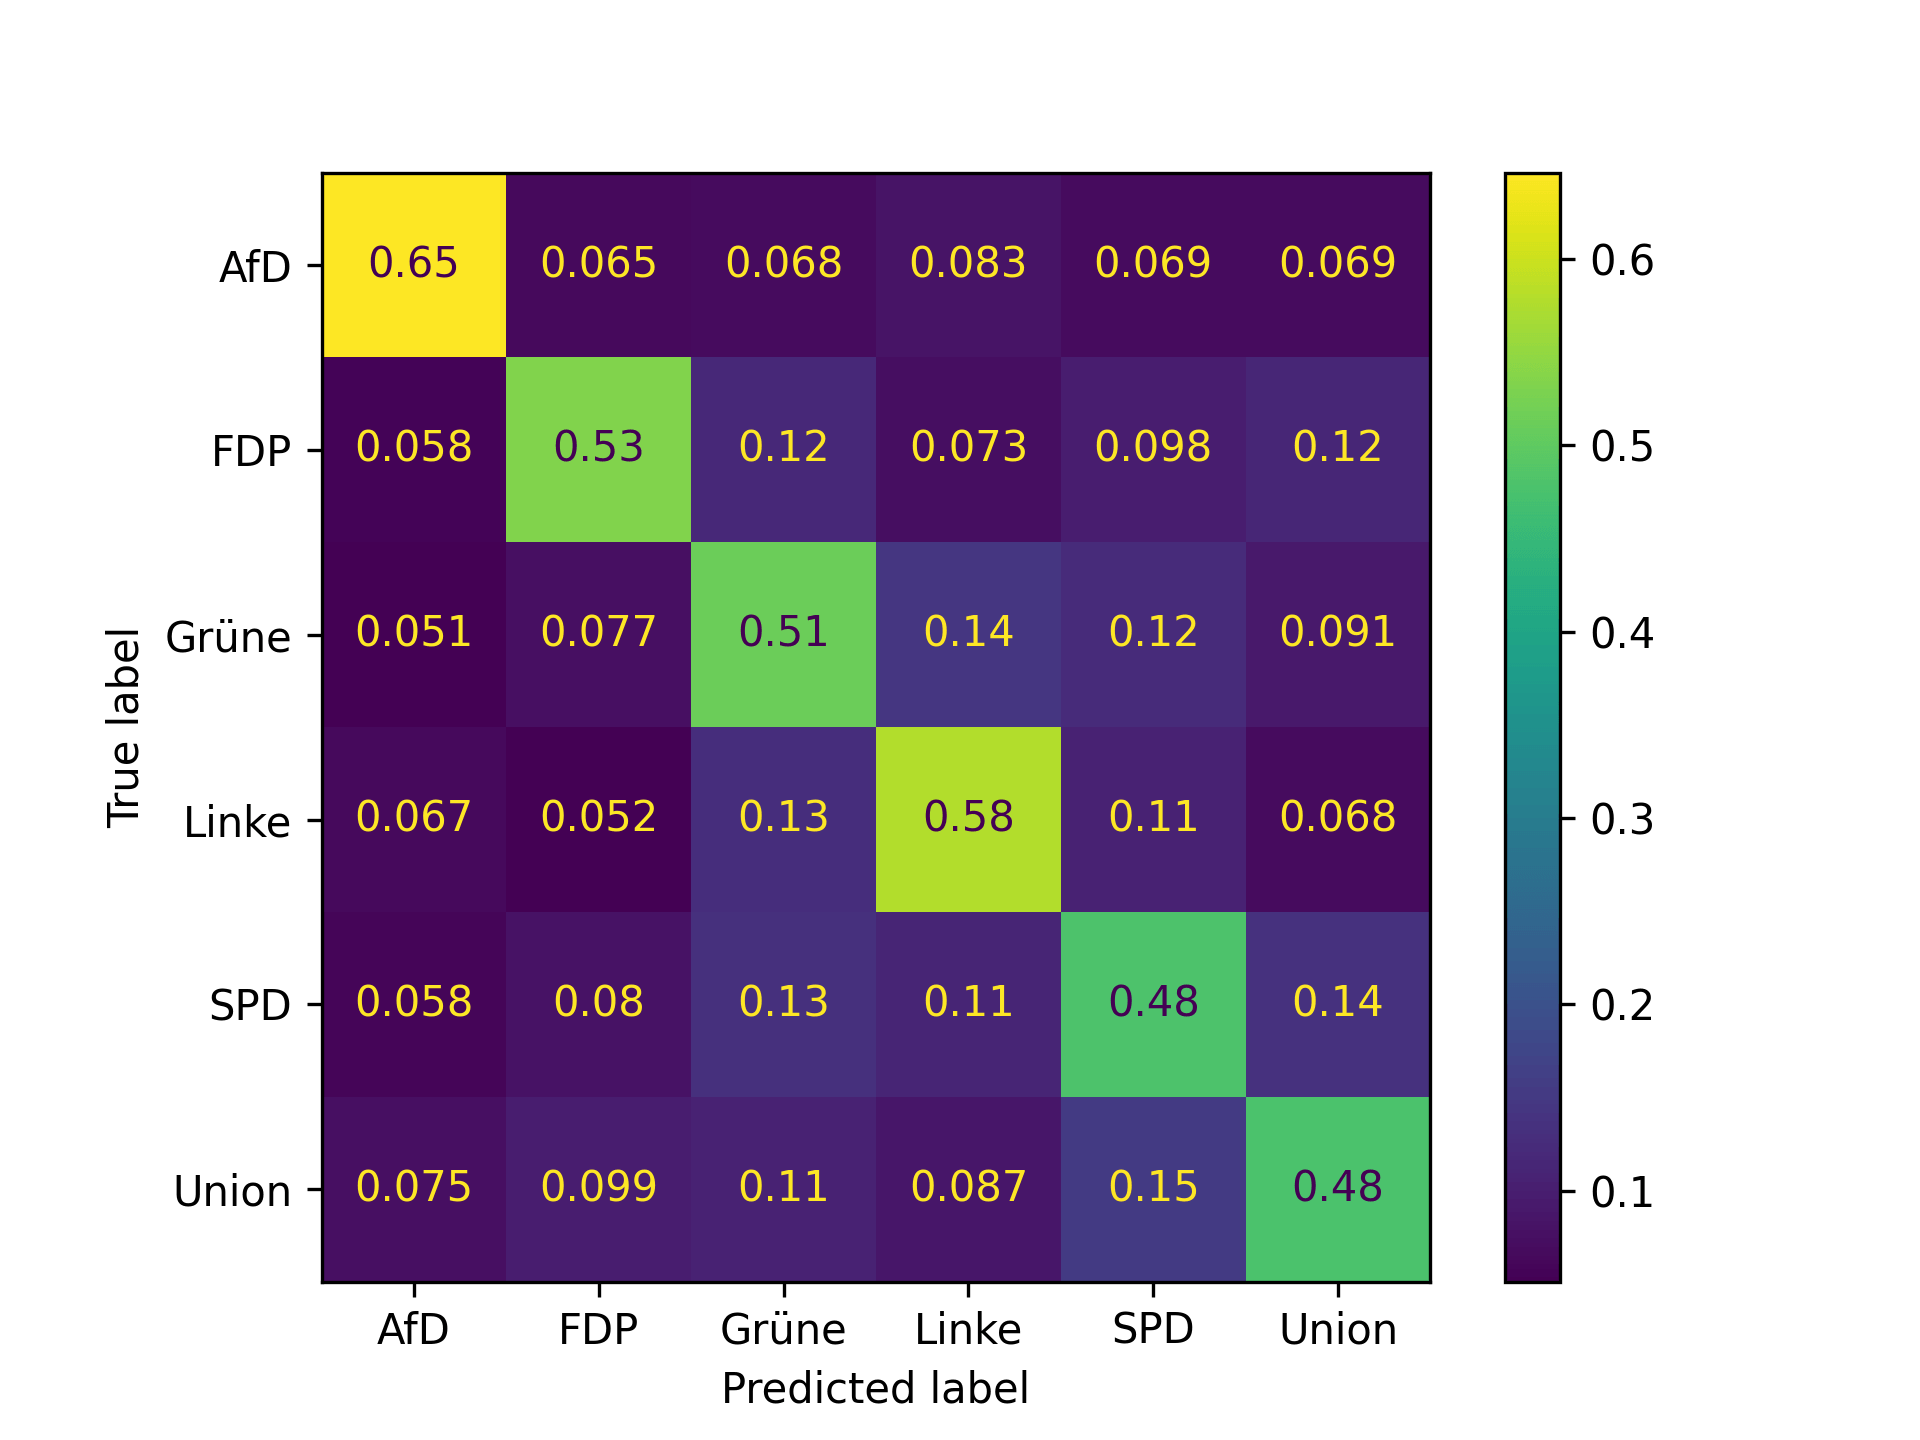
\includegraphics[width=\textwidth]{data/images/modeling/baseline/none/tweets_confusion_matrix.png}
        \caption{Tweets}
        \label{sfig:confusionMatrixBaselineTweetsUnbalanced}
    \end{subfigure}
    \hfill
    \begin{subfigure}{0.49\textwidth}
        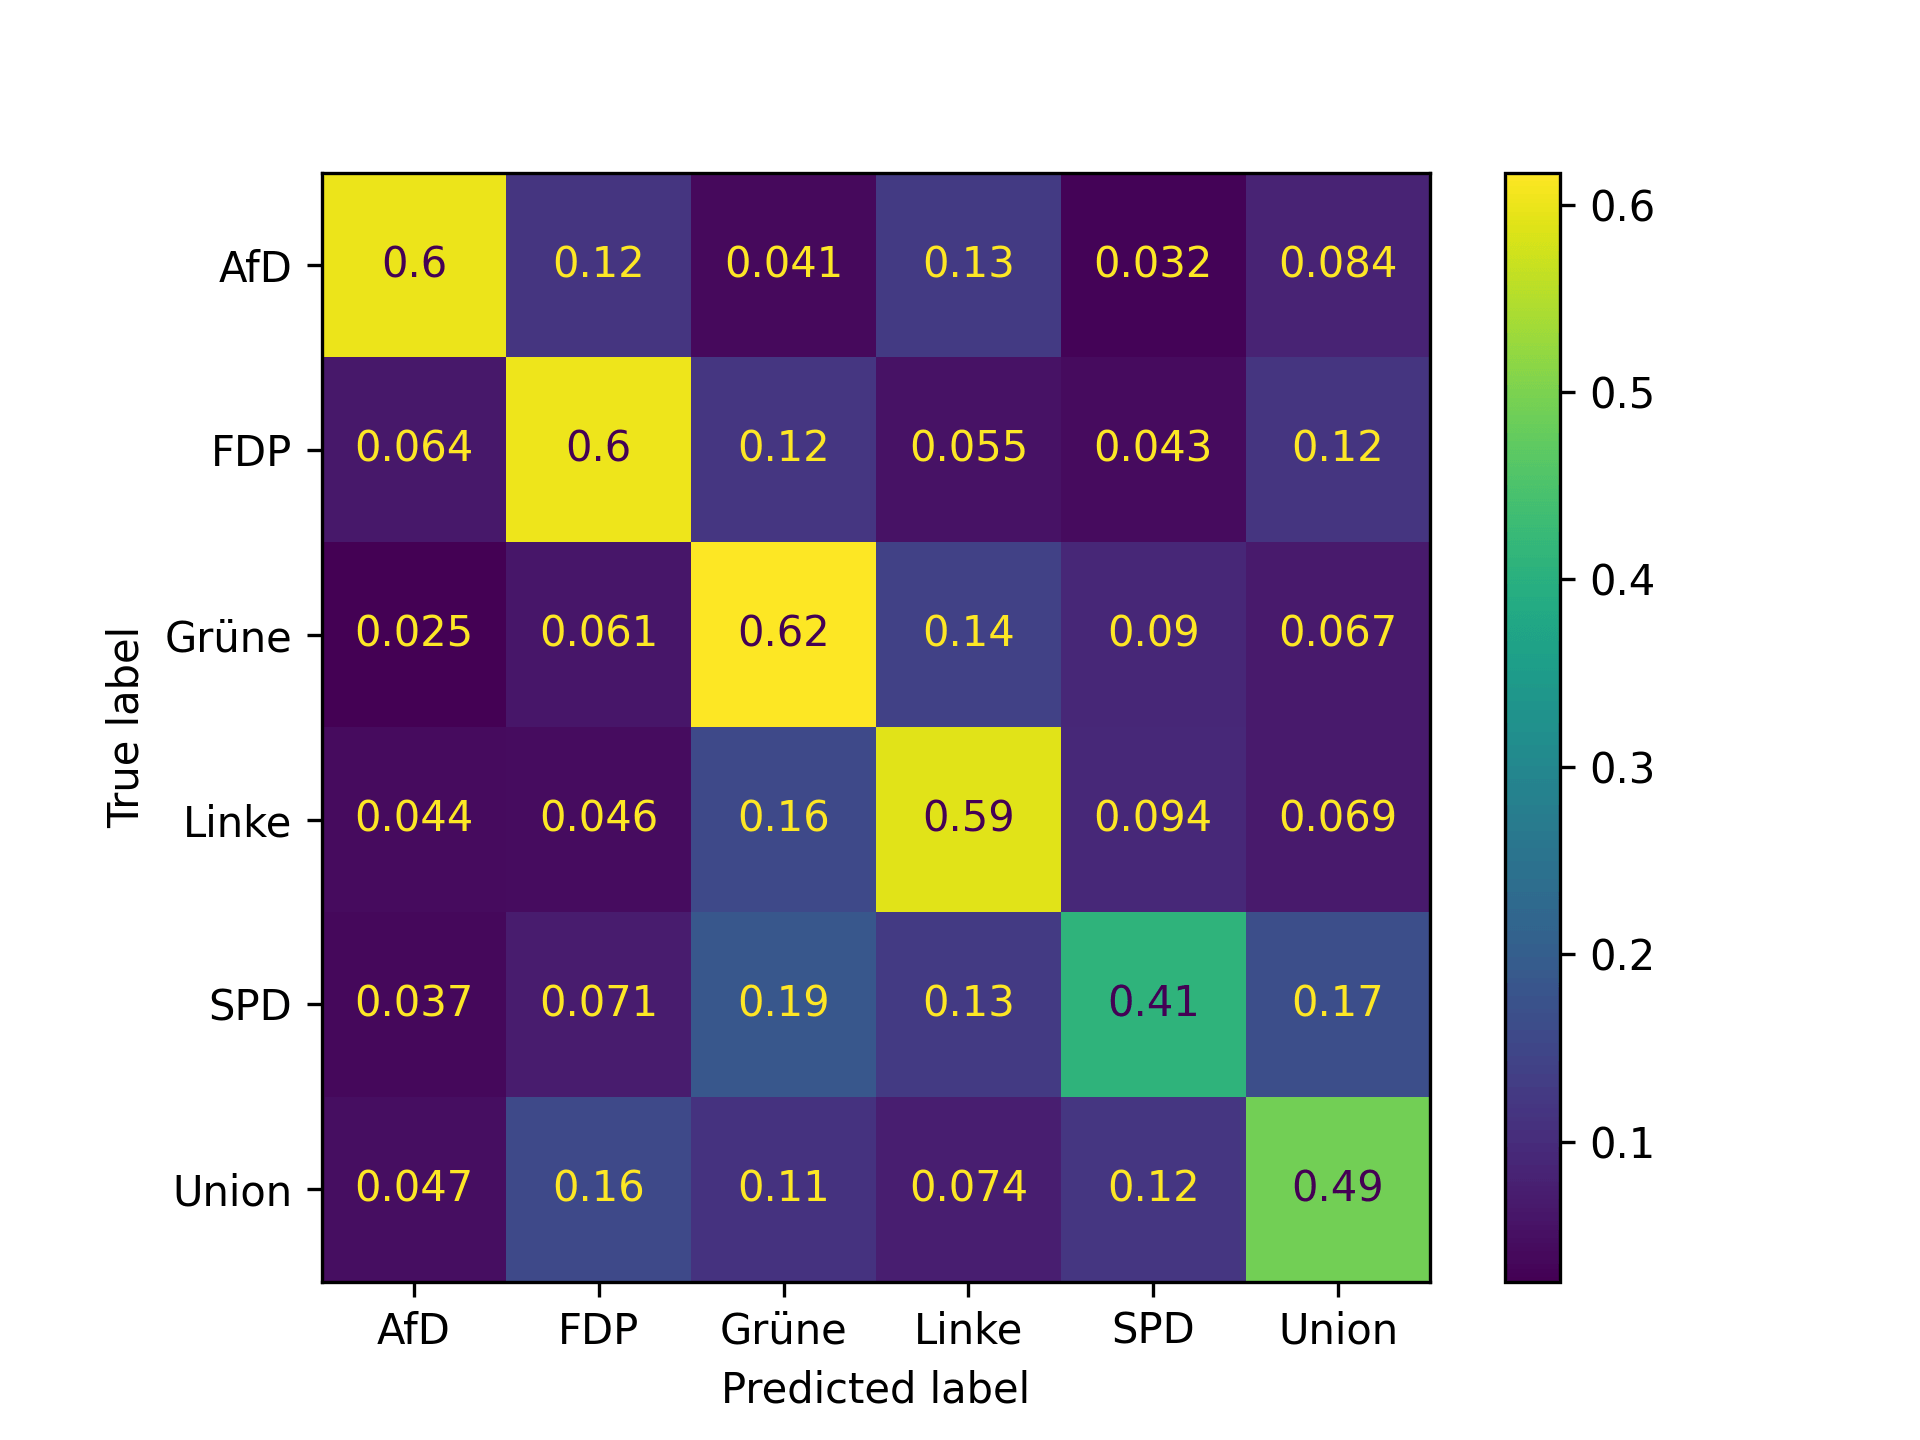
\includegraphics[width=\textwidth]{data/images/modeling/baseline/none/party_programs_confusion_matrix.png}
        \caption{Wahlprogramme}
        \label{sfig:confusionMatrixBaselineManifestUnbalanced}
    \end{subfigure}
    \hfill
    \begin{subfigure}{0.49\textwidth}
        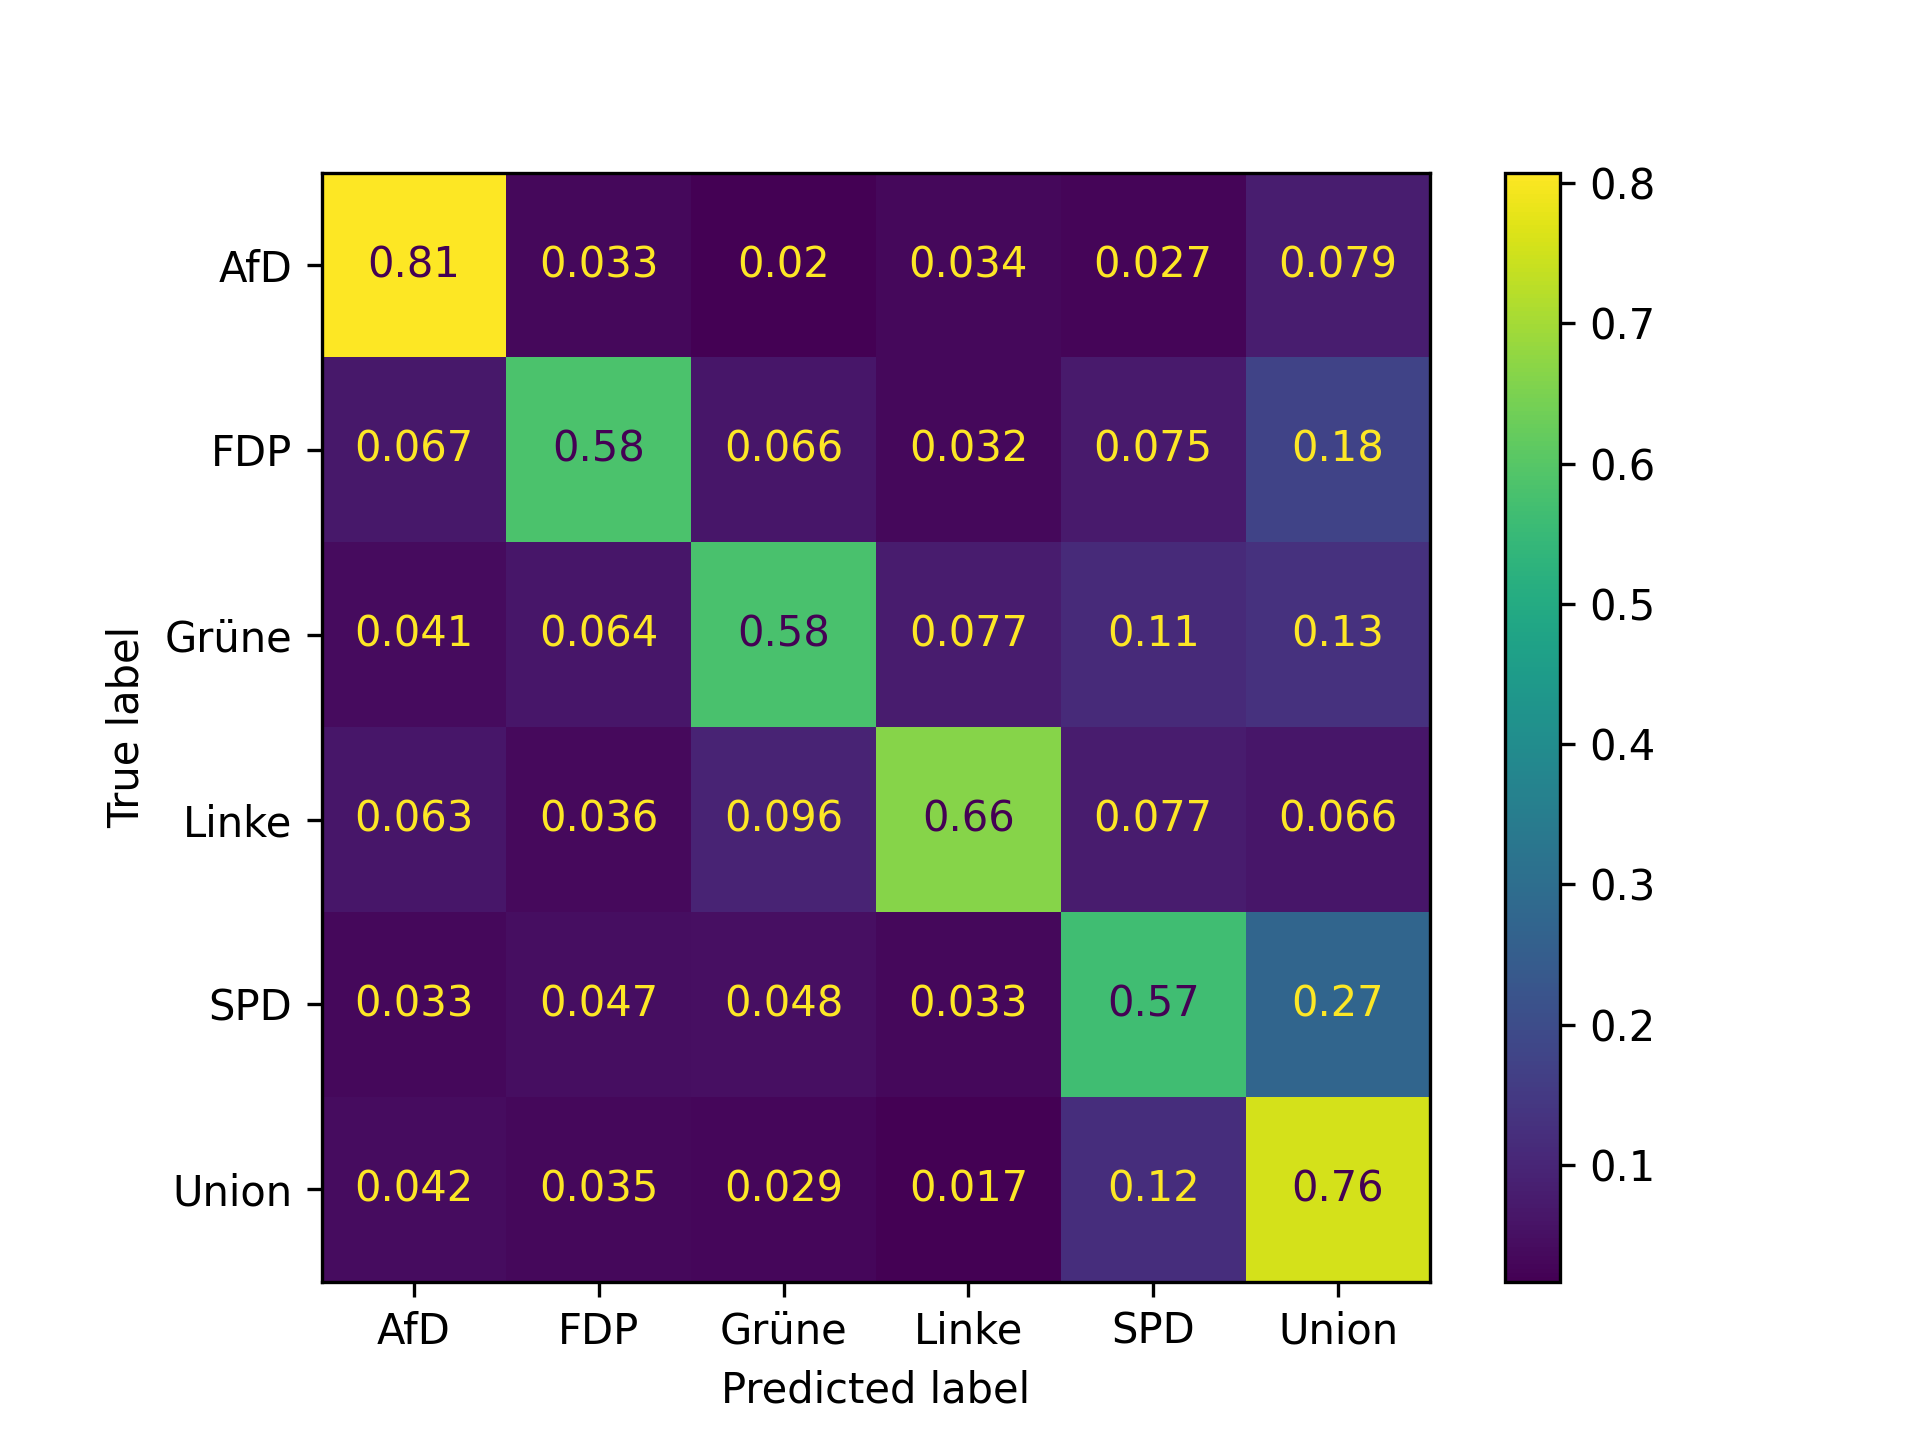
\includegraphics[width=\textwidth]{data/images/modeling/baseline/none/speeches_confusion_matrix.png}
        \caption{Reden}
        \label{sfig:confusionMatrixBaselineSpeechesUnbalanced}
    \end{subfigure}
    \caption{Konfusionsmatrizen für Lineare \acs{SVC} und \acs{TF-IDF} auf unausgeglichenen Datensätzen} \label{fig:confusionMatrixBaselineUnbalanced}
\end{figure}

\subsection*{fastText}

\begin{figure}[H]
    \begin{subfigure}{0.5\textwidth}
        \centering
        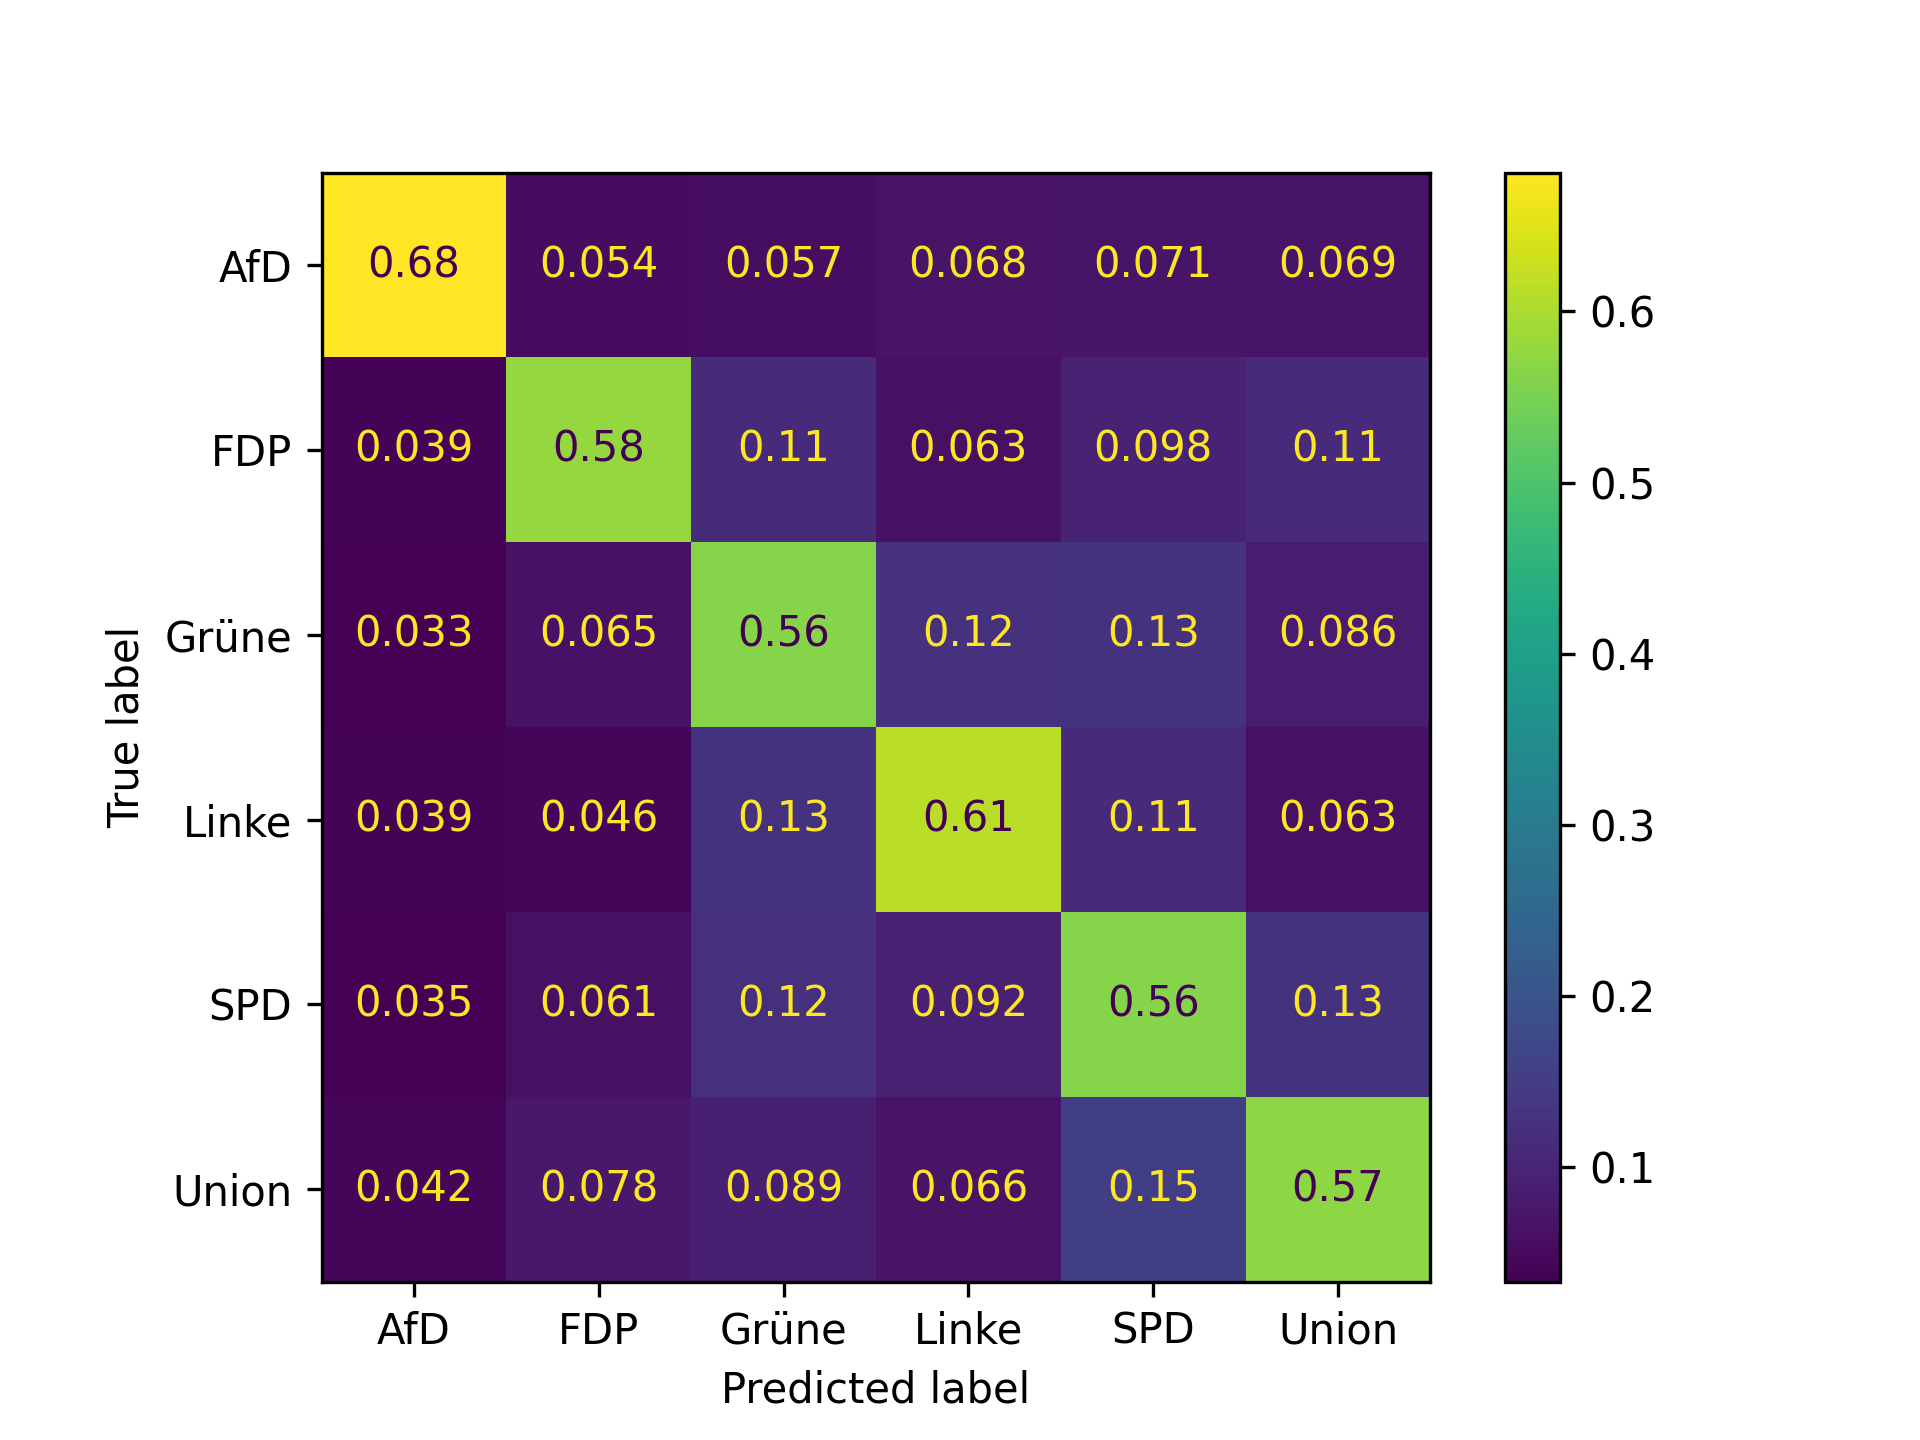
\includegraphics[width=0.9\textwidth]{data/images/modeling/fasttext/none/tweets_confusion_matrix.png}
        \caption{Tweets} \label{sfig:confusionMatrixFastTextTweetsUnbalanced}
    \end{subfigure}
    \hfill
    \begin{subfigure}{0.5\textwidth}
        \centering
        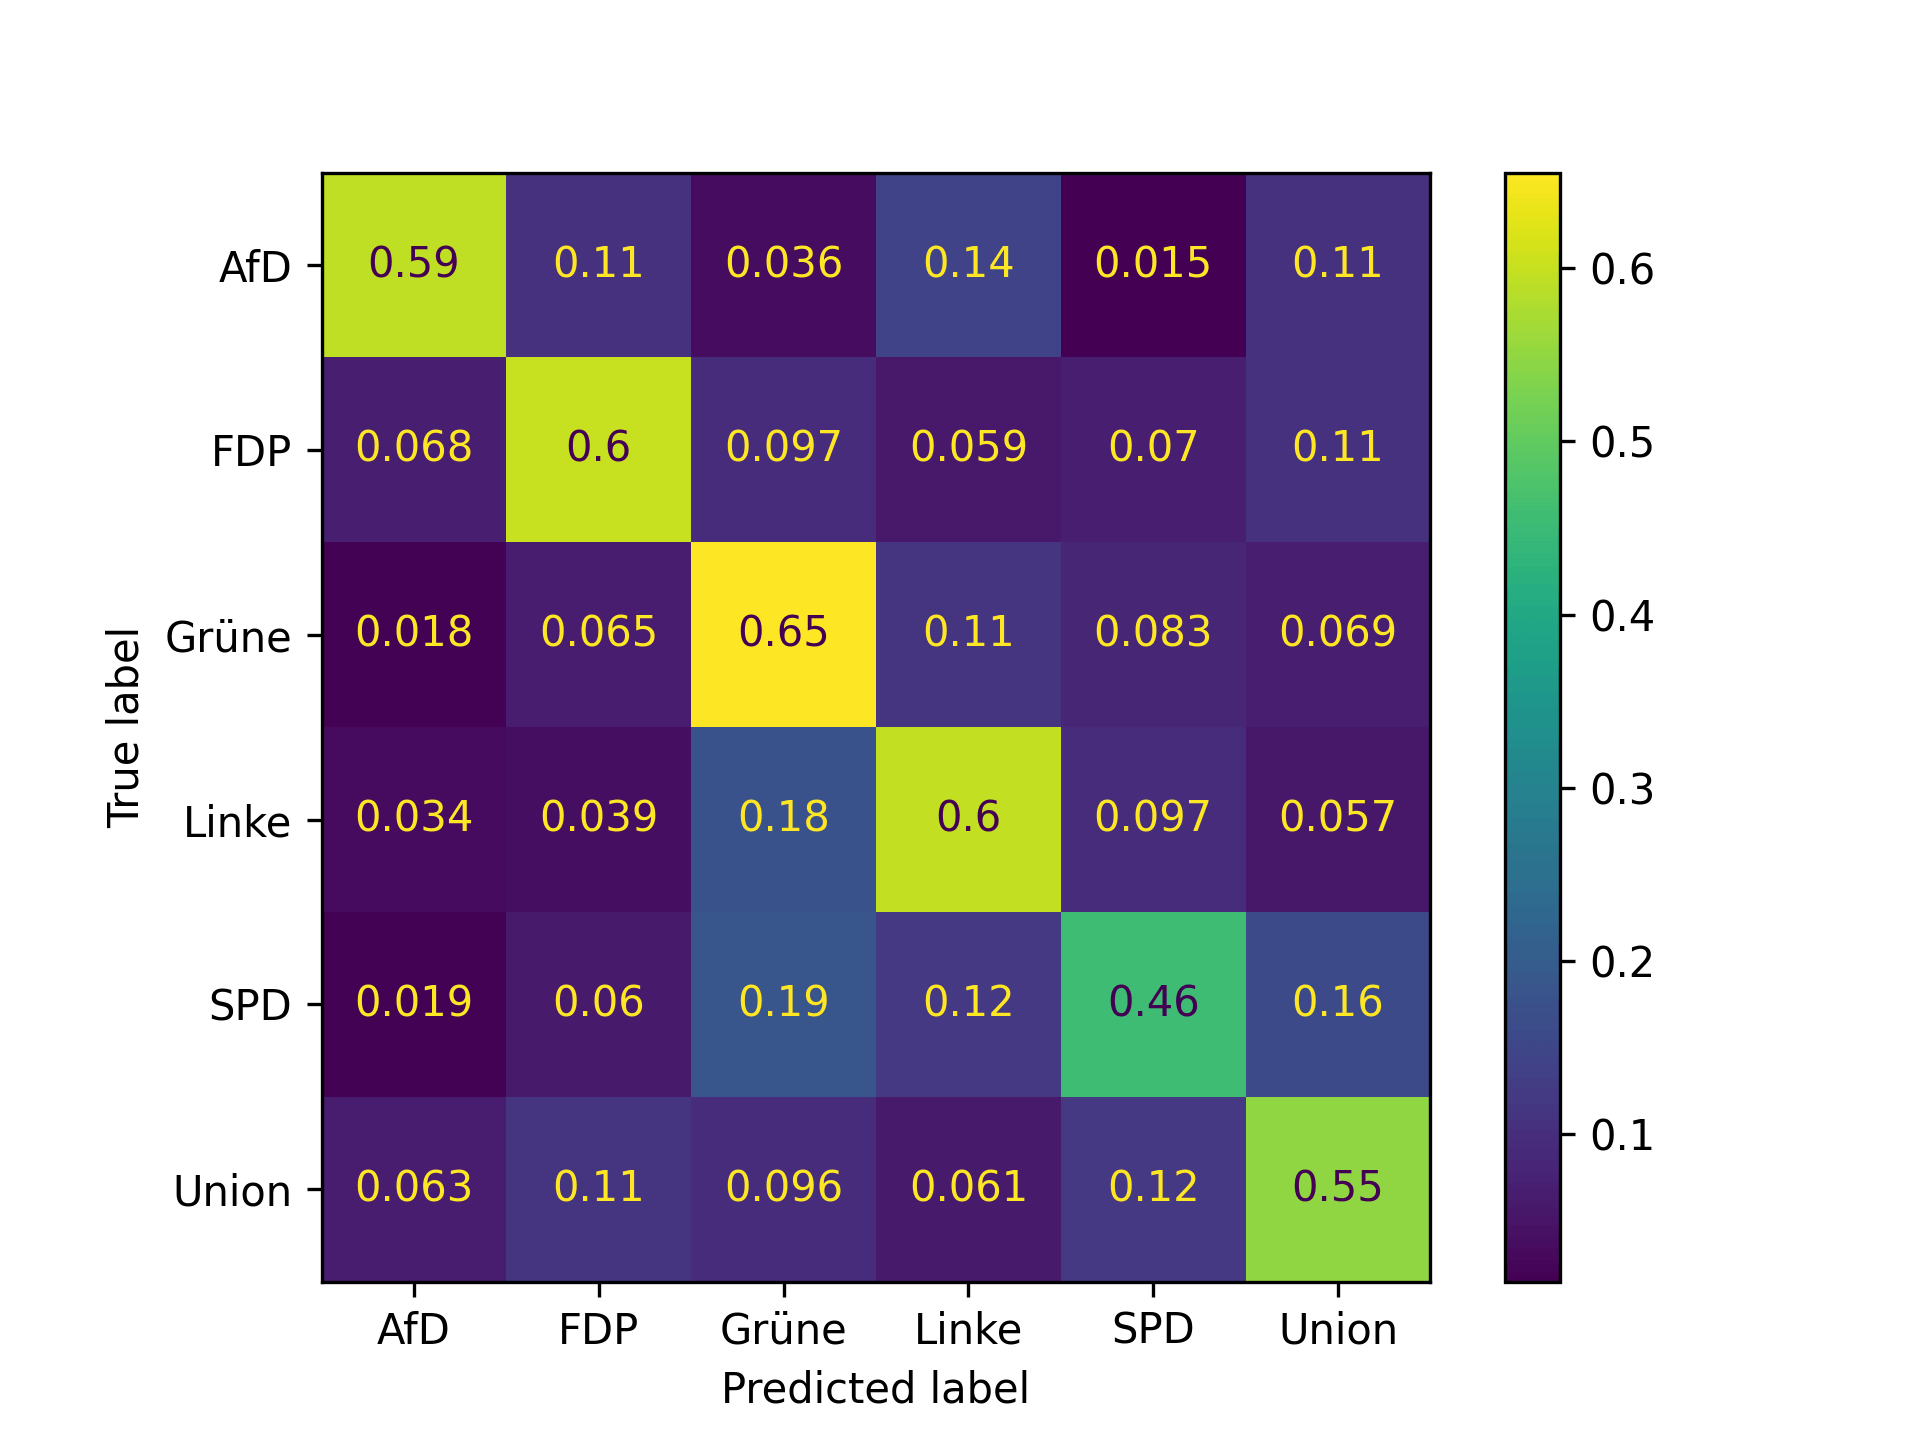
\includegraphics[width=0.9\textwidth]{data/images/modeling/fasttext/none/party_programs_confusion_matrix.png}
        \caption{Wahlprogramme} \label{sfig:confusionMatrixFastTextManifestUnbalanced}
    \end{subfigure}
    \hfill
    \begin{subfigure}{0.5\textwidth}
        \centering
        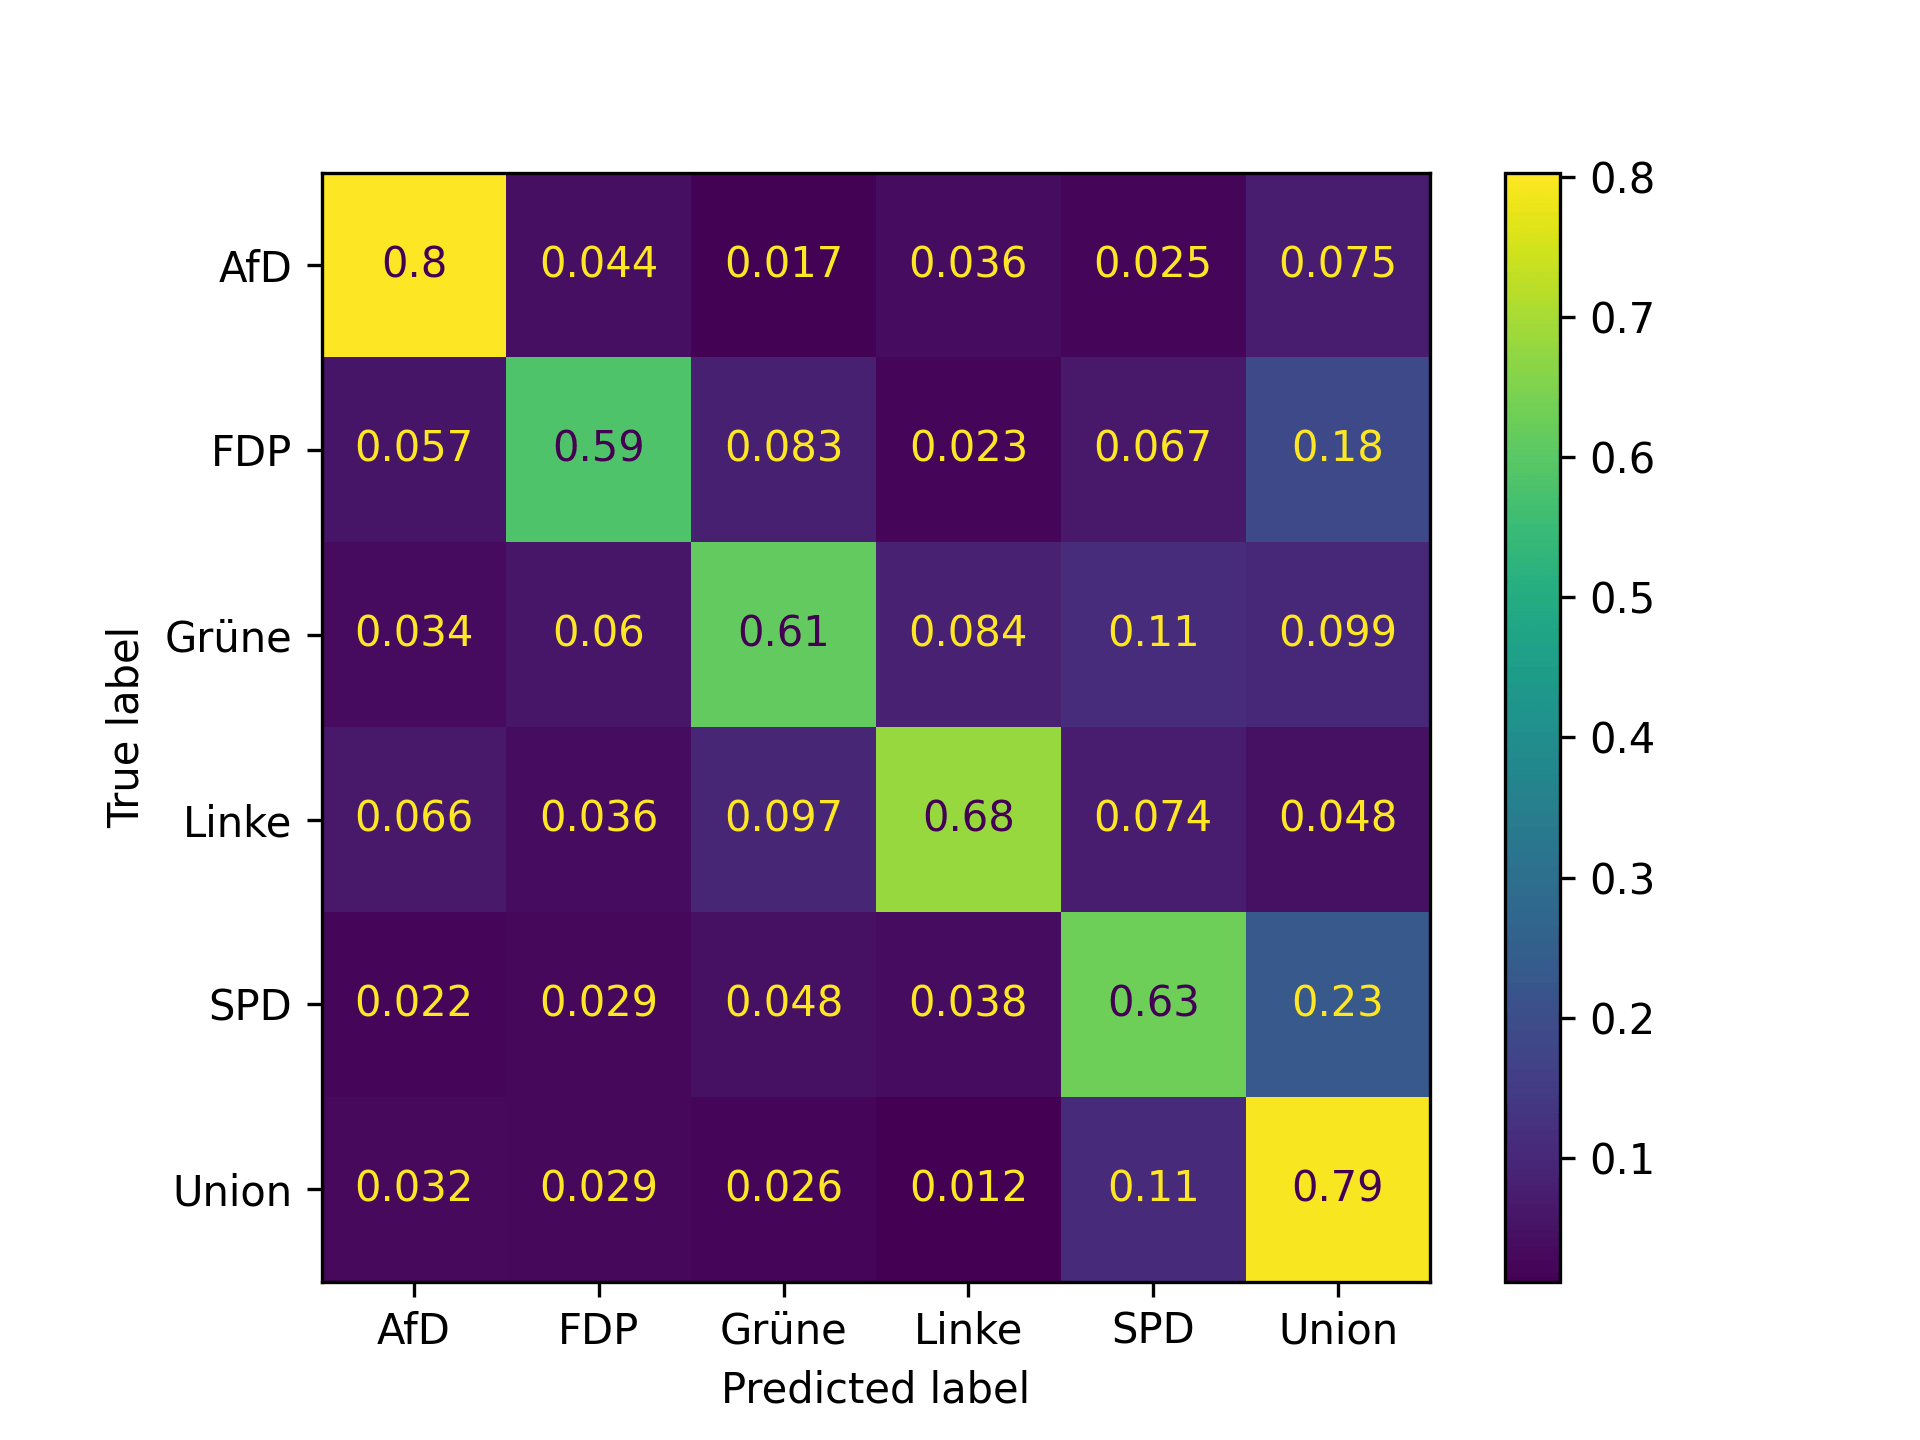
\includegraphics[width=0.9\textwidth]{data/images/modeling/fasttext/none/speeches_confusion_matrix.png}
        \caption{Reden} \label{sfig:confusionMatrixFastTextSpeechesUnbalanced}
    \end{subfigure}
    \hfill
    \begin{subfigure}{0.49\textwidth}
        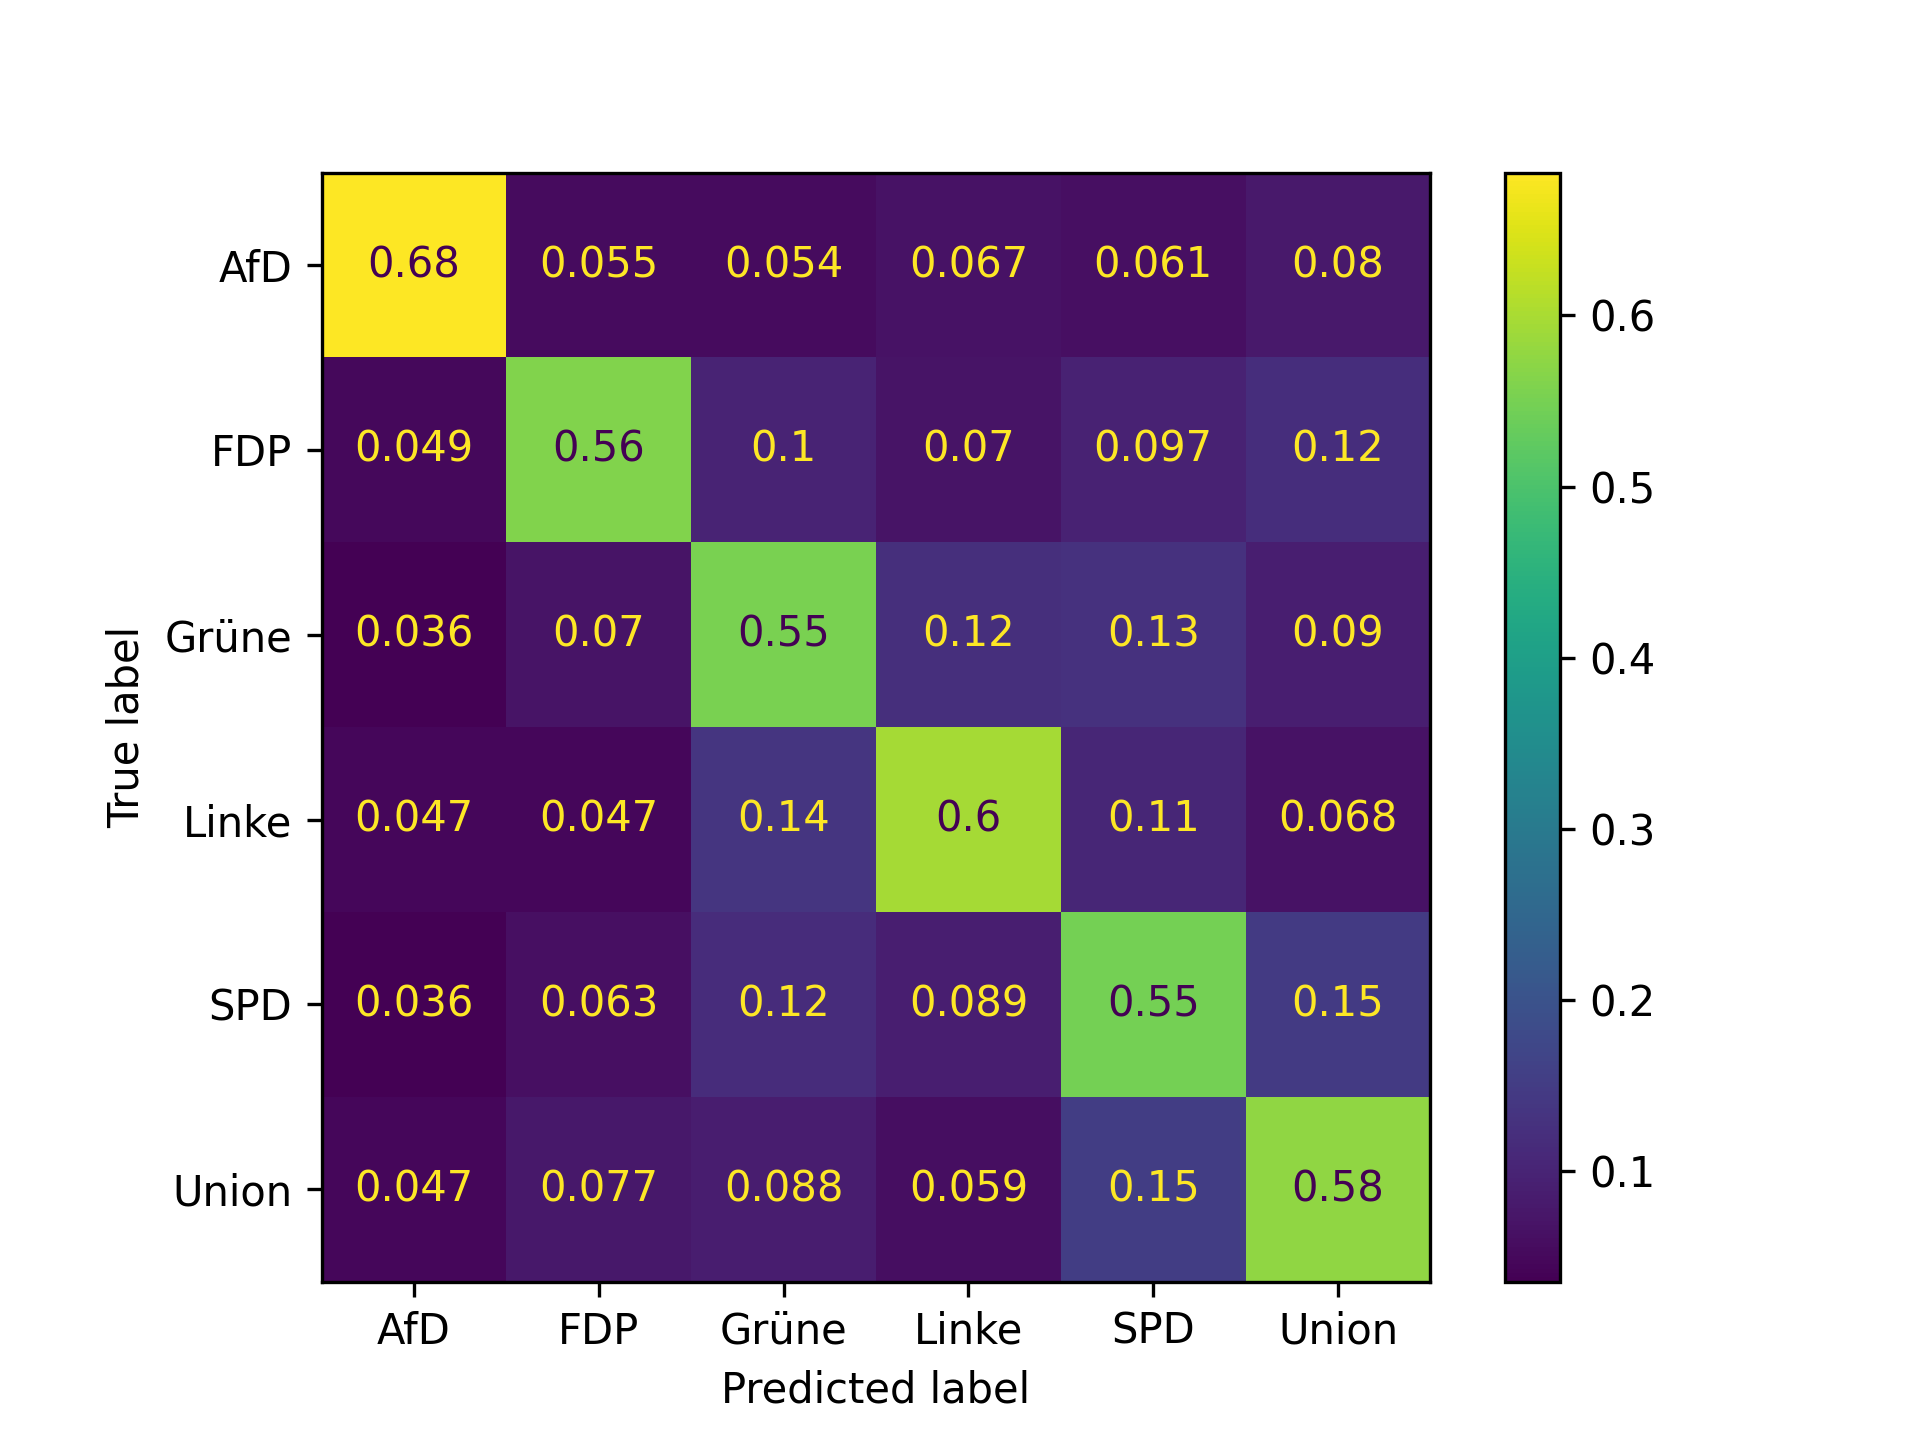
\includegraphics[width=\textwidth]{data/images/modeling/fasttext/none/all_confusion_matrix.png}
        \caption{Kombiniert} \label{sfig:confusionMatrixFastTextAllUnbalanced}
    \end{subfigure}
    \caption{Konfusionsmatrizen für \ft mit Bigrammen (\(n = \num{2}\)) auf unausgeglichenen Datensätzen} \label{fig:unbalancedConfusionMatrixFastText}
\end{figure}

\subsection*{Multi-Layer Perceptron}

\begin{figure}[H]
    \centering
    \begin{subfigure}{0.49\textwidth}
        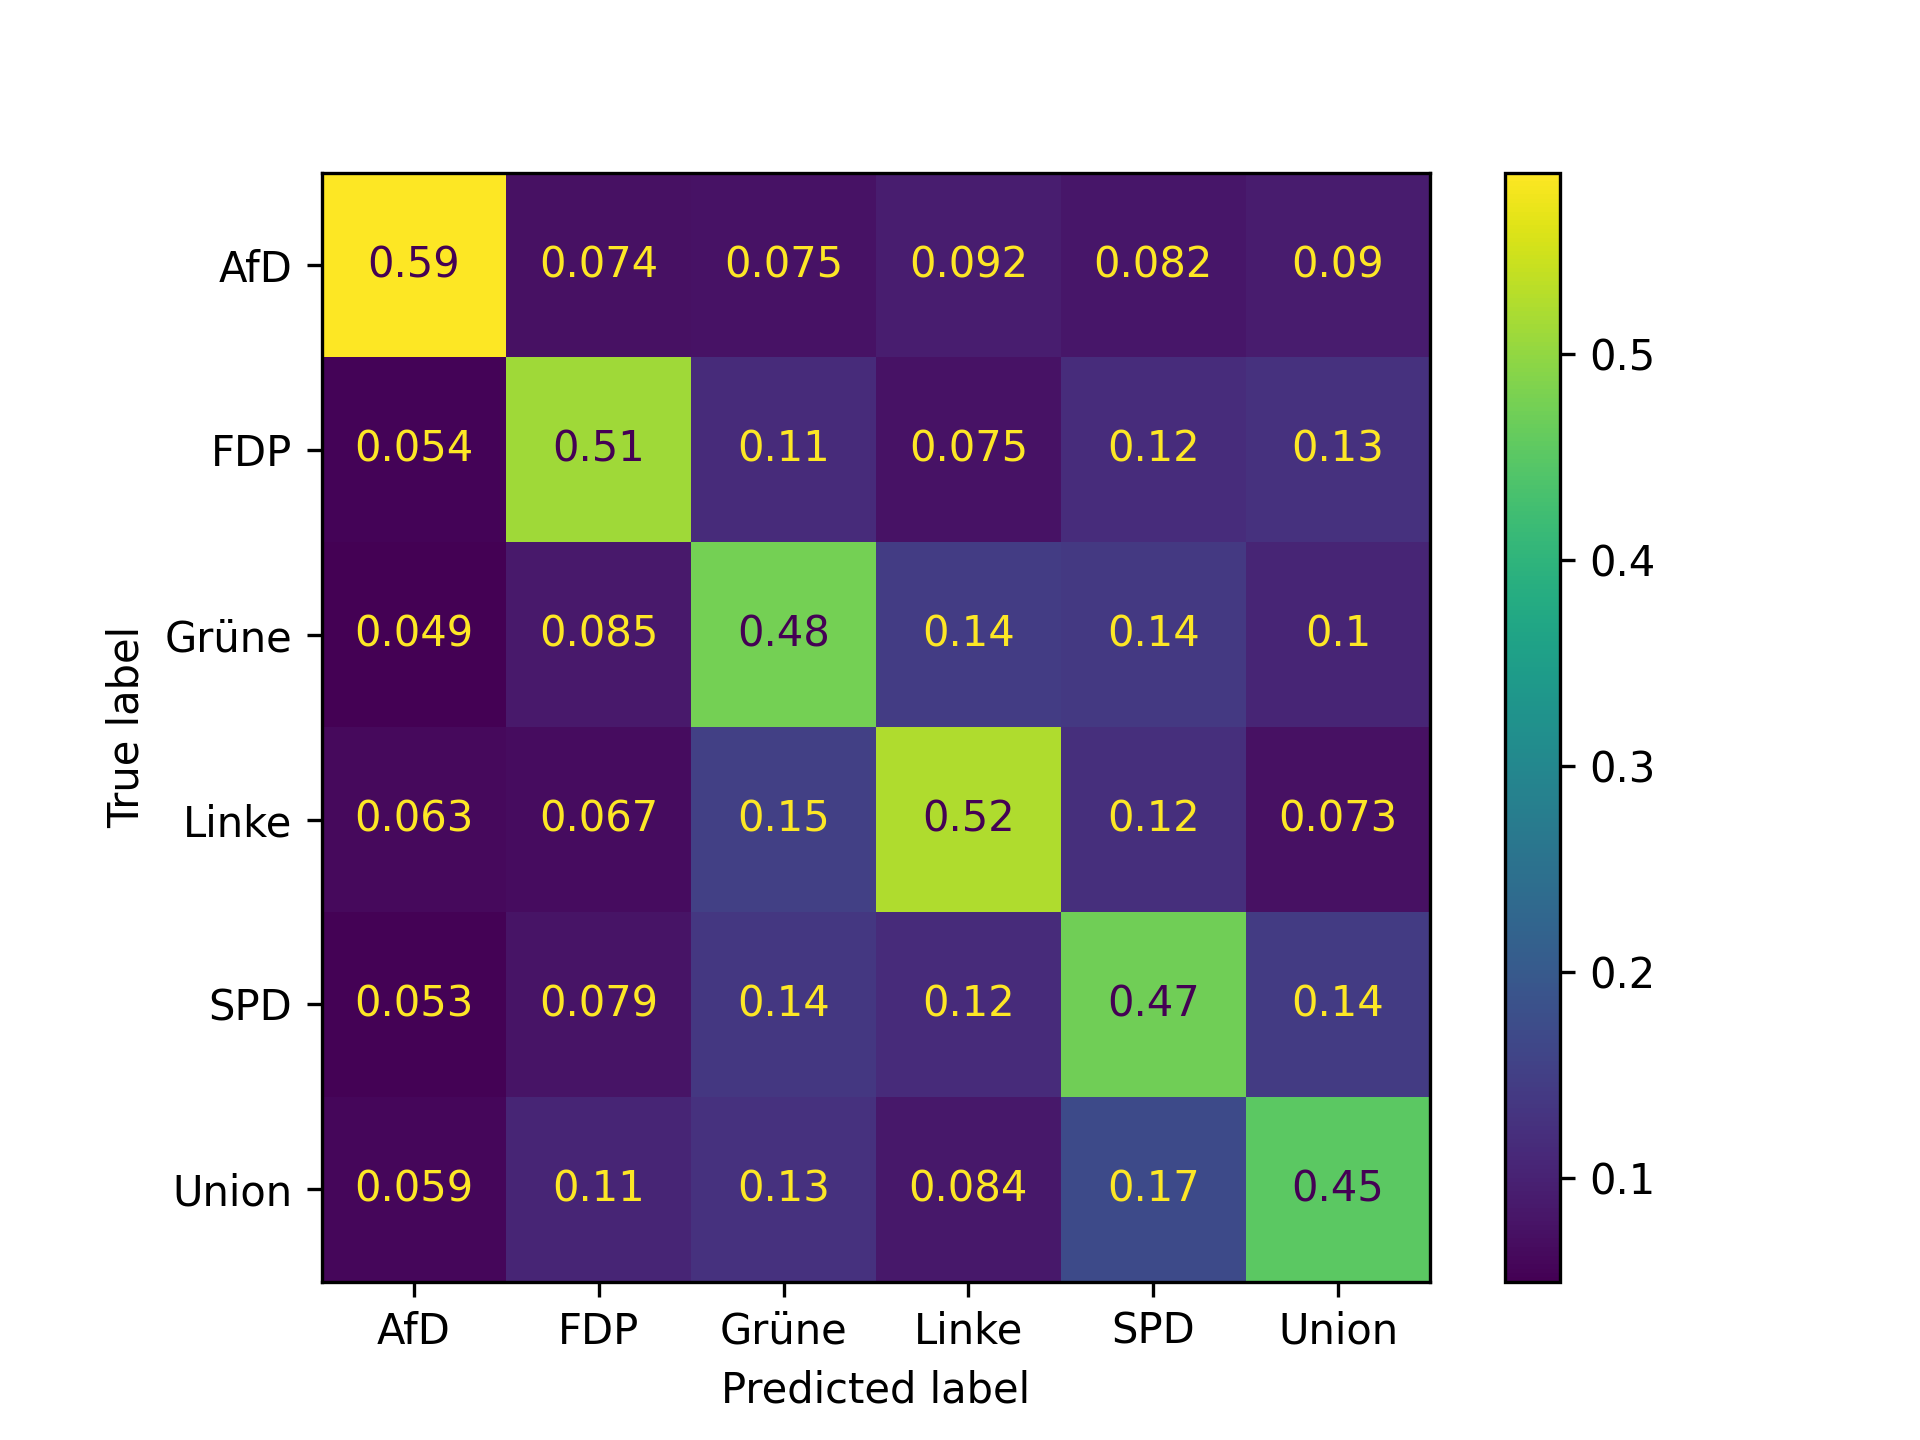
\includegraphics[width=\textwidth]{data/images/modeling/mlp/none/tweets_confusion_matrix.png}
        \caption{Tweets, \ac{BoW}}
        \label{sfig:confusionMatrixMlpTweetsUnbalanced}
    \end{subfigure}
    \hfill
    \begin{subfigure}{0.49\textwidth}
        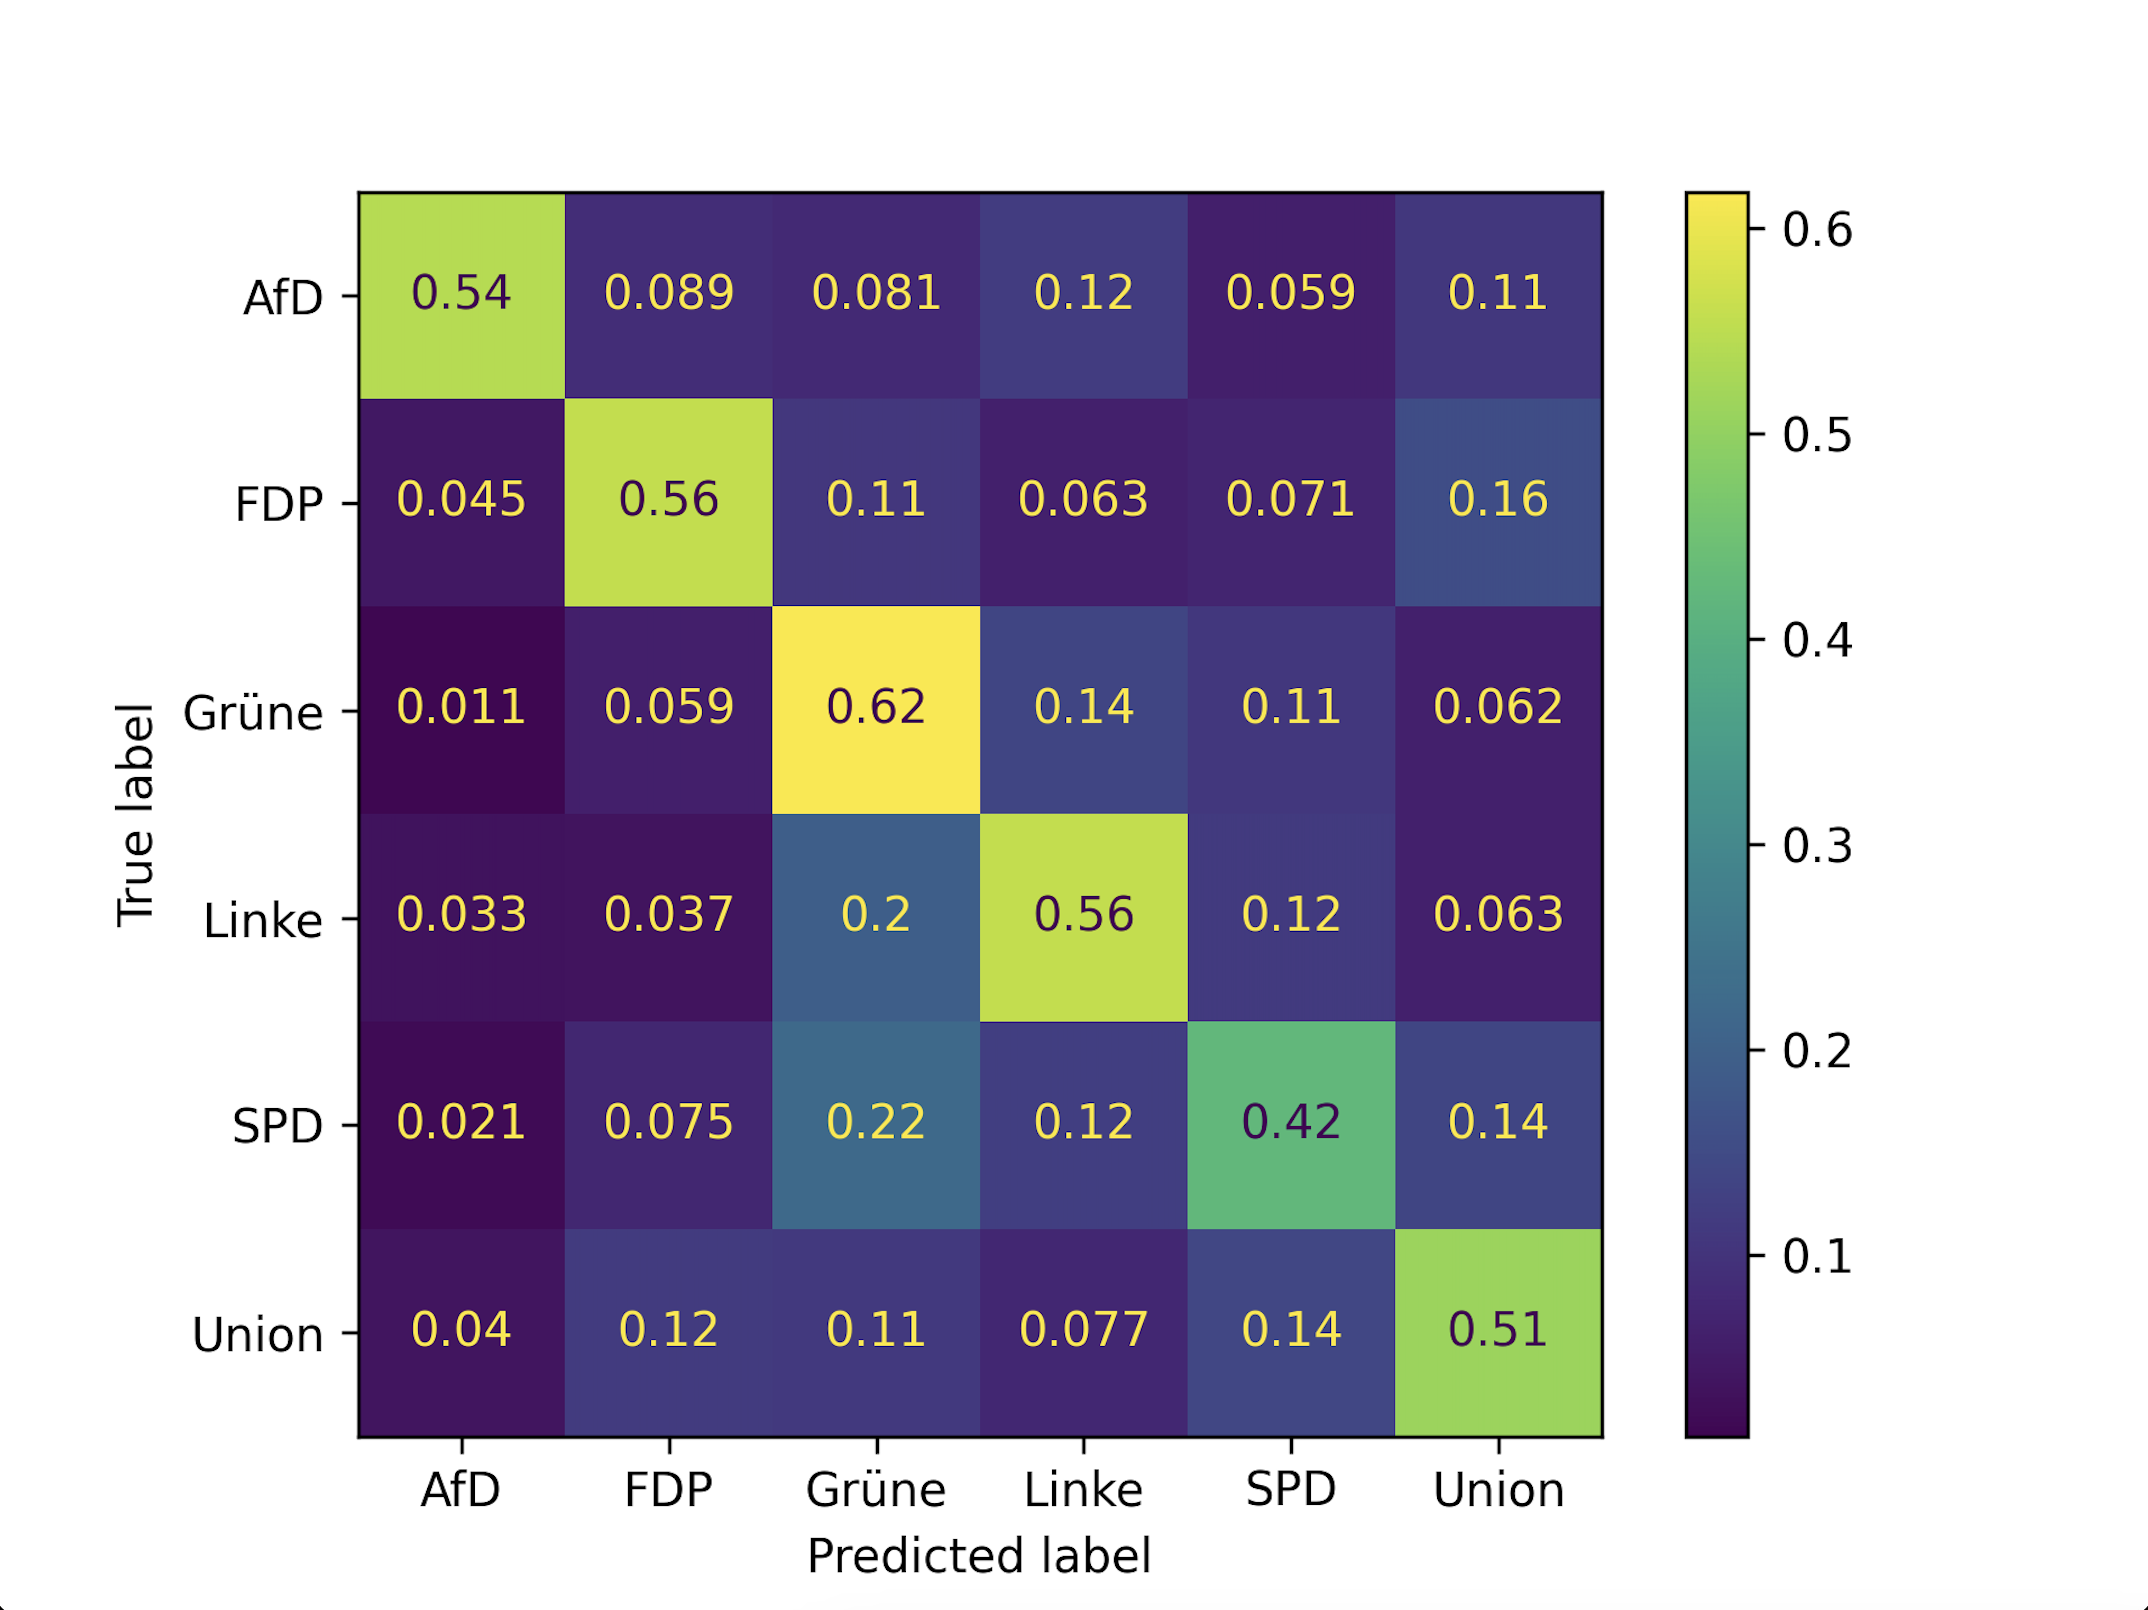
\includegraphics[width=\textwidth]{data/images/modeling/mlp/none/party_programs_confusion_matrix.png}
        \caption{Wahlprogramme, \ac{TF-IDF}}
        \label{sfig:confusionMatrixMlpManifestUnbalanced}
    \end{subfigure}
    \hfill
    \begin{subfigure}{0.49\textwidth}
        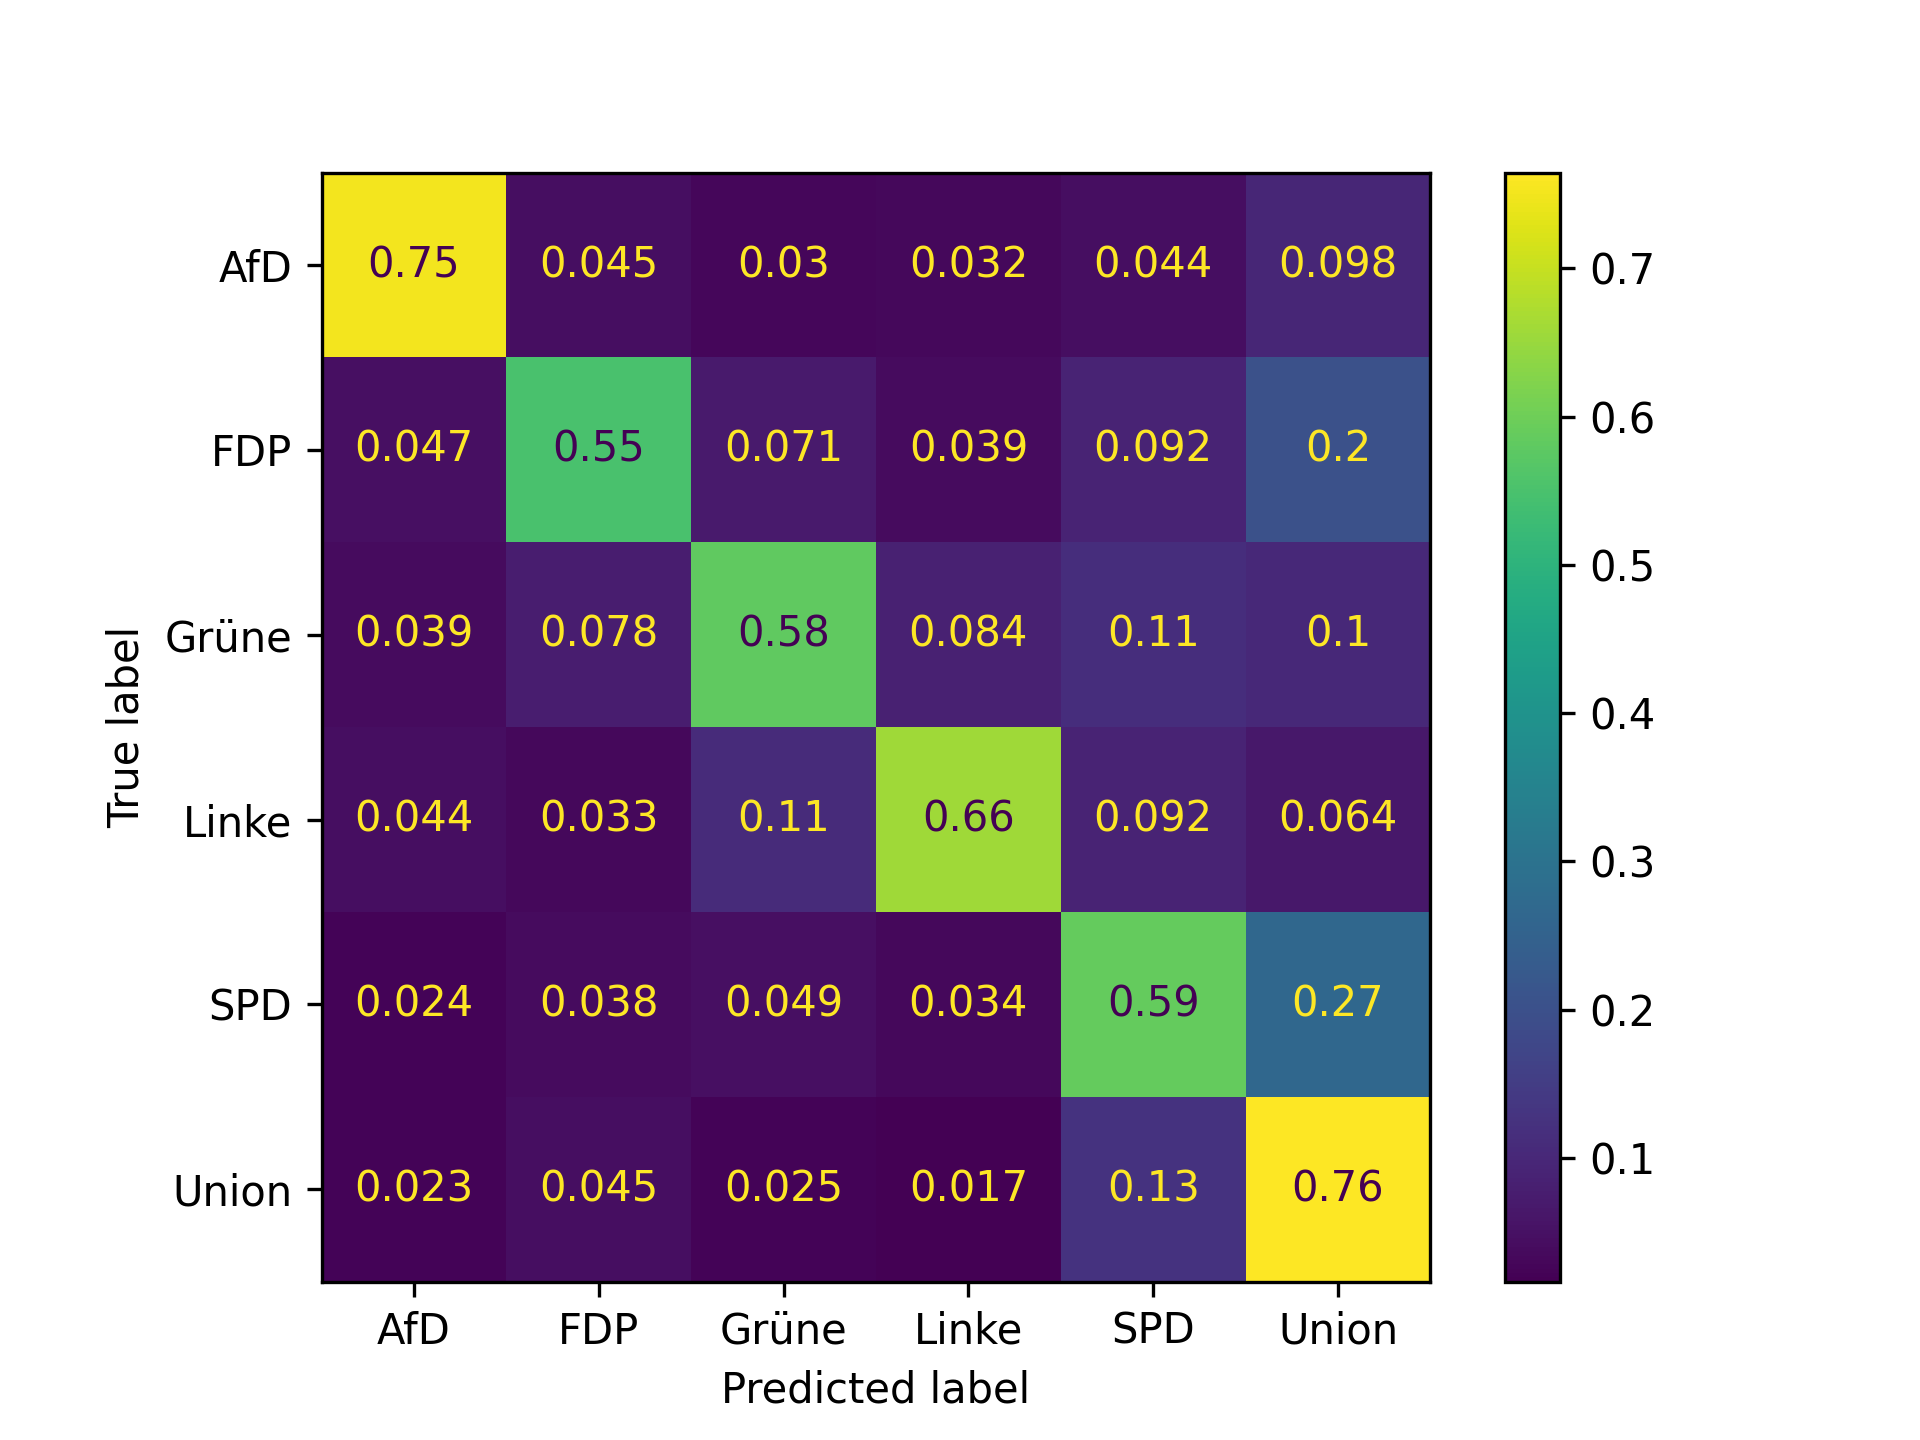
\includegraphics[width=\textwidth]{data/images/modeling/mlp/none/speeches_confusion_matrix.png}
        \caption{Reden, \ac{BoW}}
        \label{sfig:confusionMatrixMlpSpeechesUnbalanced}
    \end{subfigure}
    \caption{Konfusionsmatrizen für das \acs{MLP}-Modell auf unausgeglichenen Datensätzen} \label{fig:confusionMatrixMlpUnbalanced}
\end{figure}

\subsection*{CNN}

\begin{figure}[H]
    \centering
    \begin{subfigure}{0.49\textwidth}
        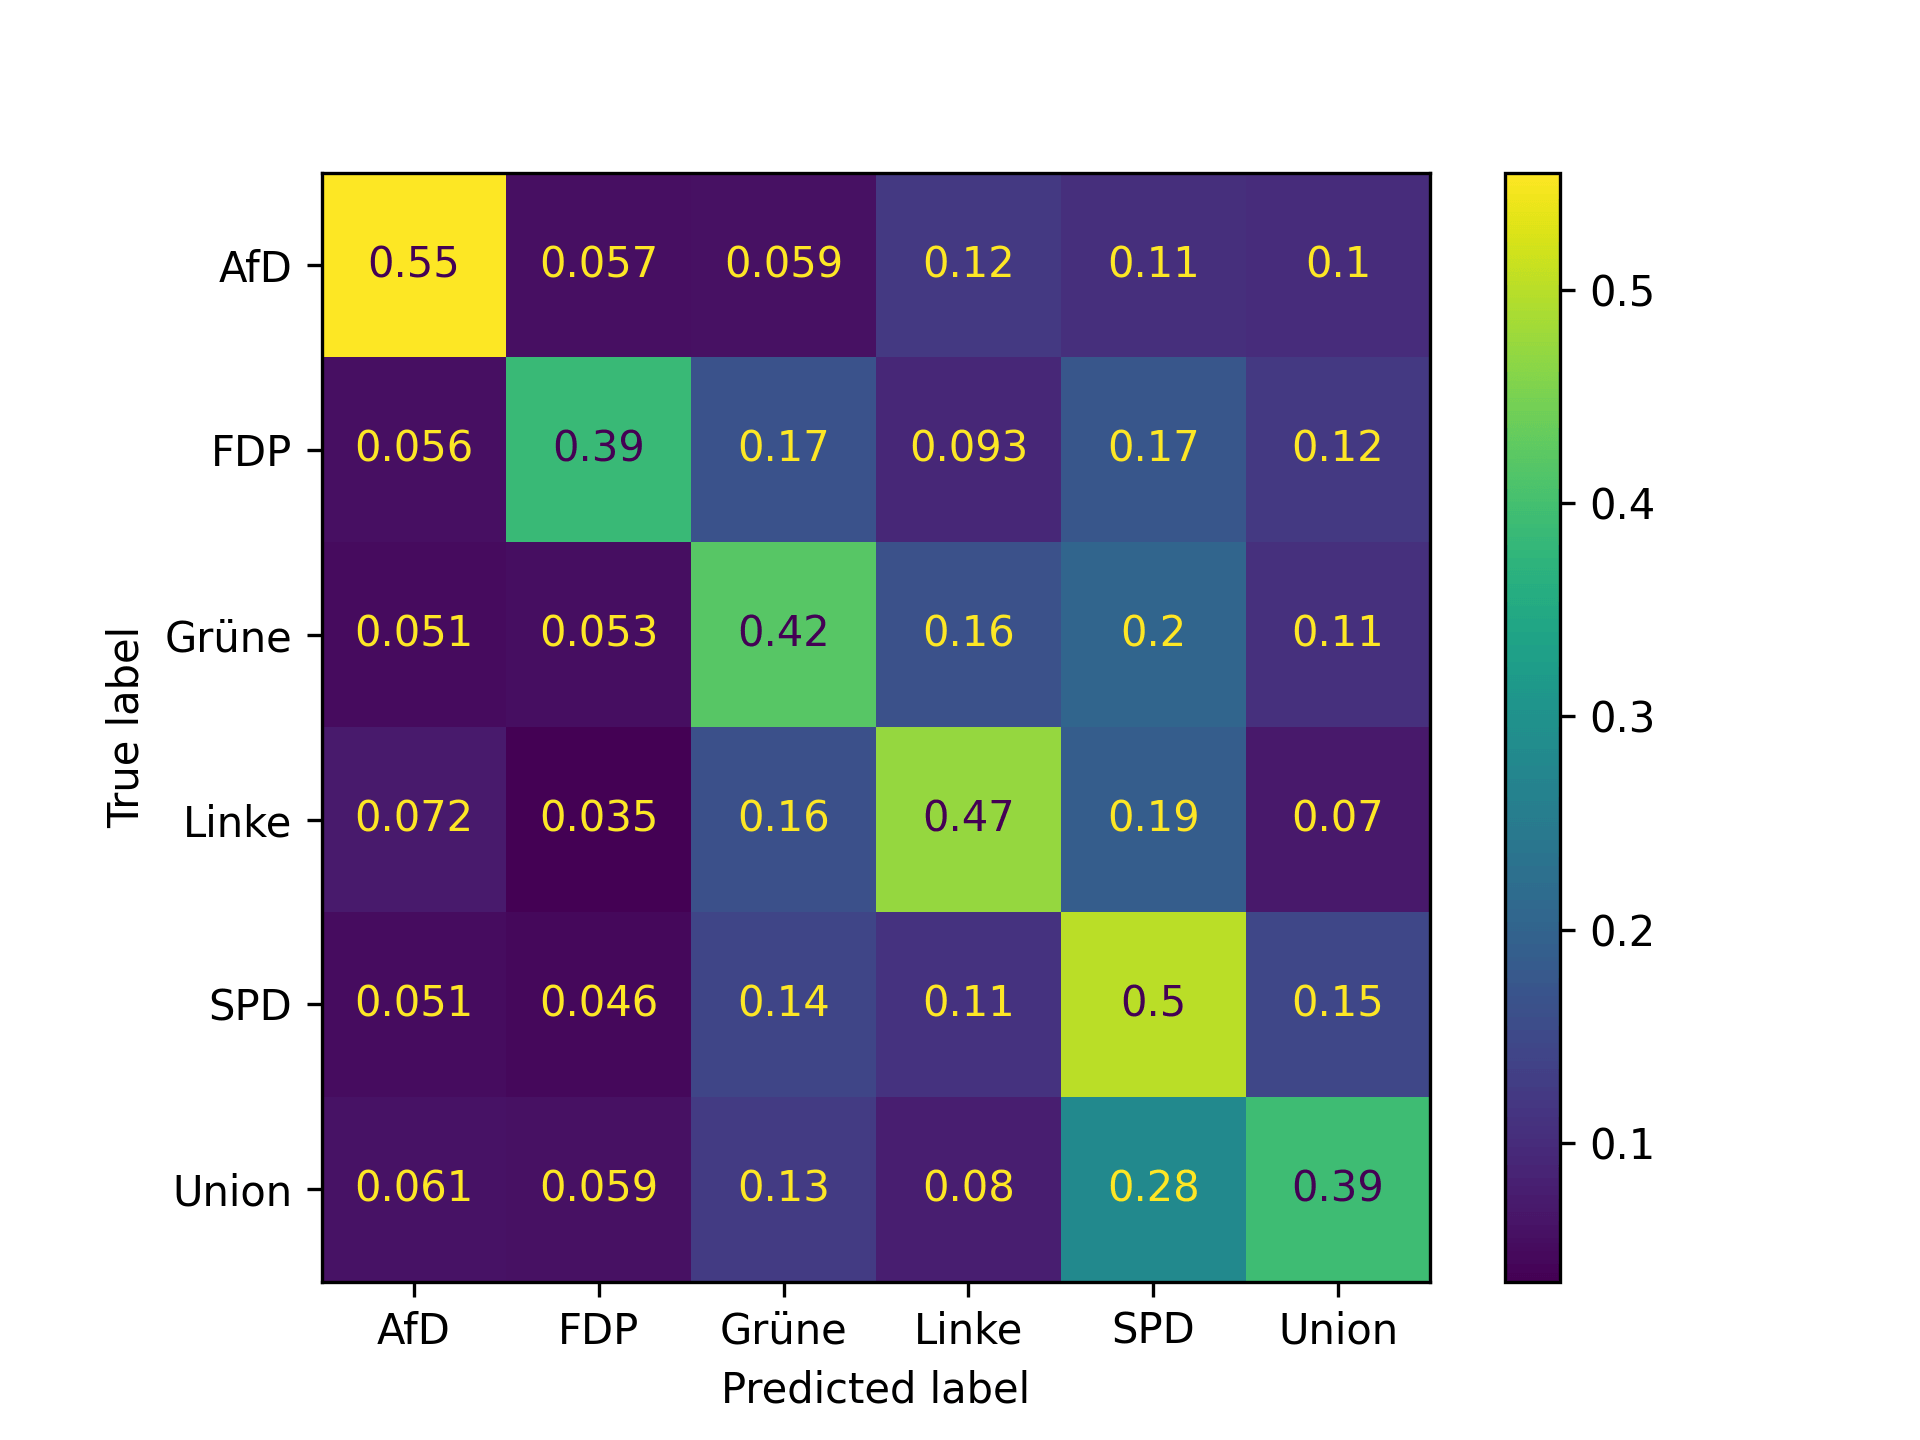
\includegraphics[width=\textwidth]{data/images/modeling/cnn/none/tweets_confusion_matrix.png}
        \caption{Tweets}
        \label{sfig:confusionMatrixCnnTweetsUnbalanced}
    \end{subfigure}
    \hfill
    \begin{subfigure}{0.49\textwidth}
        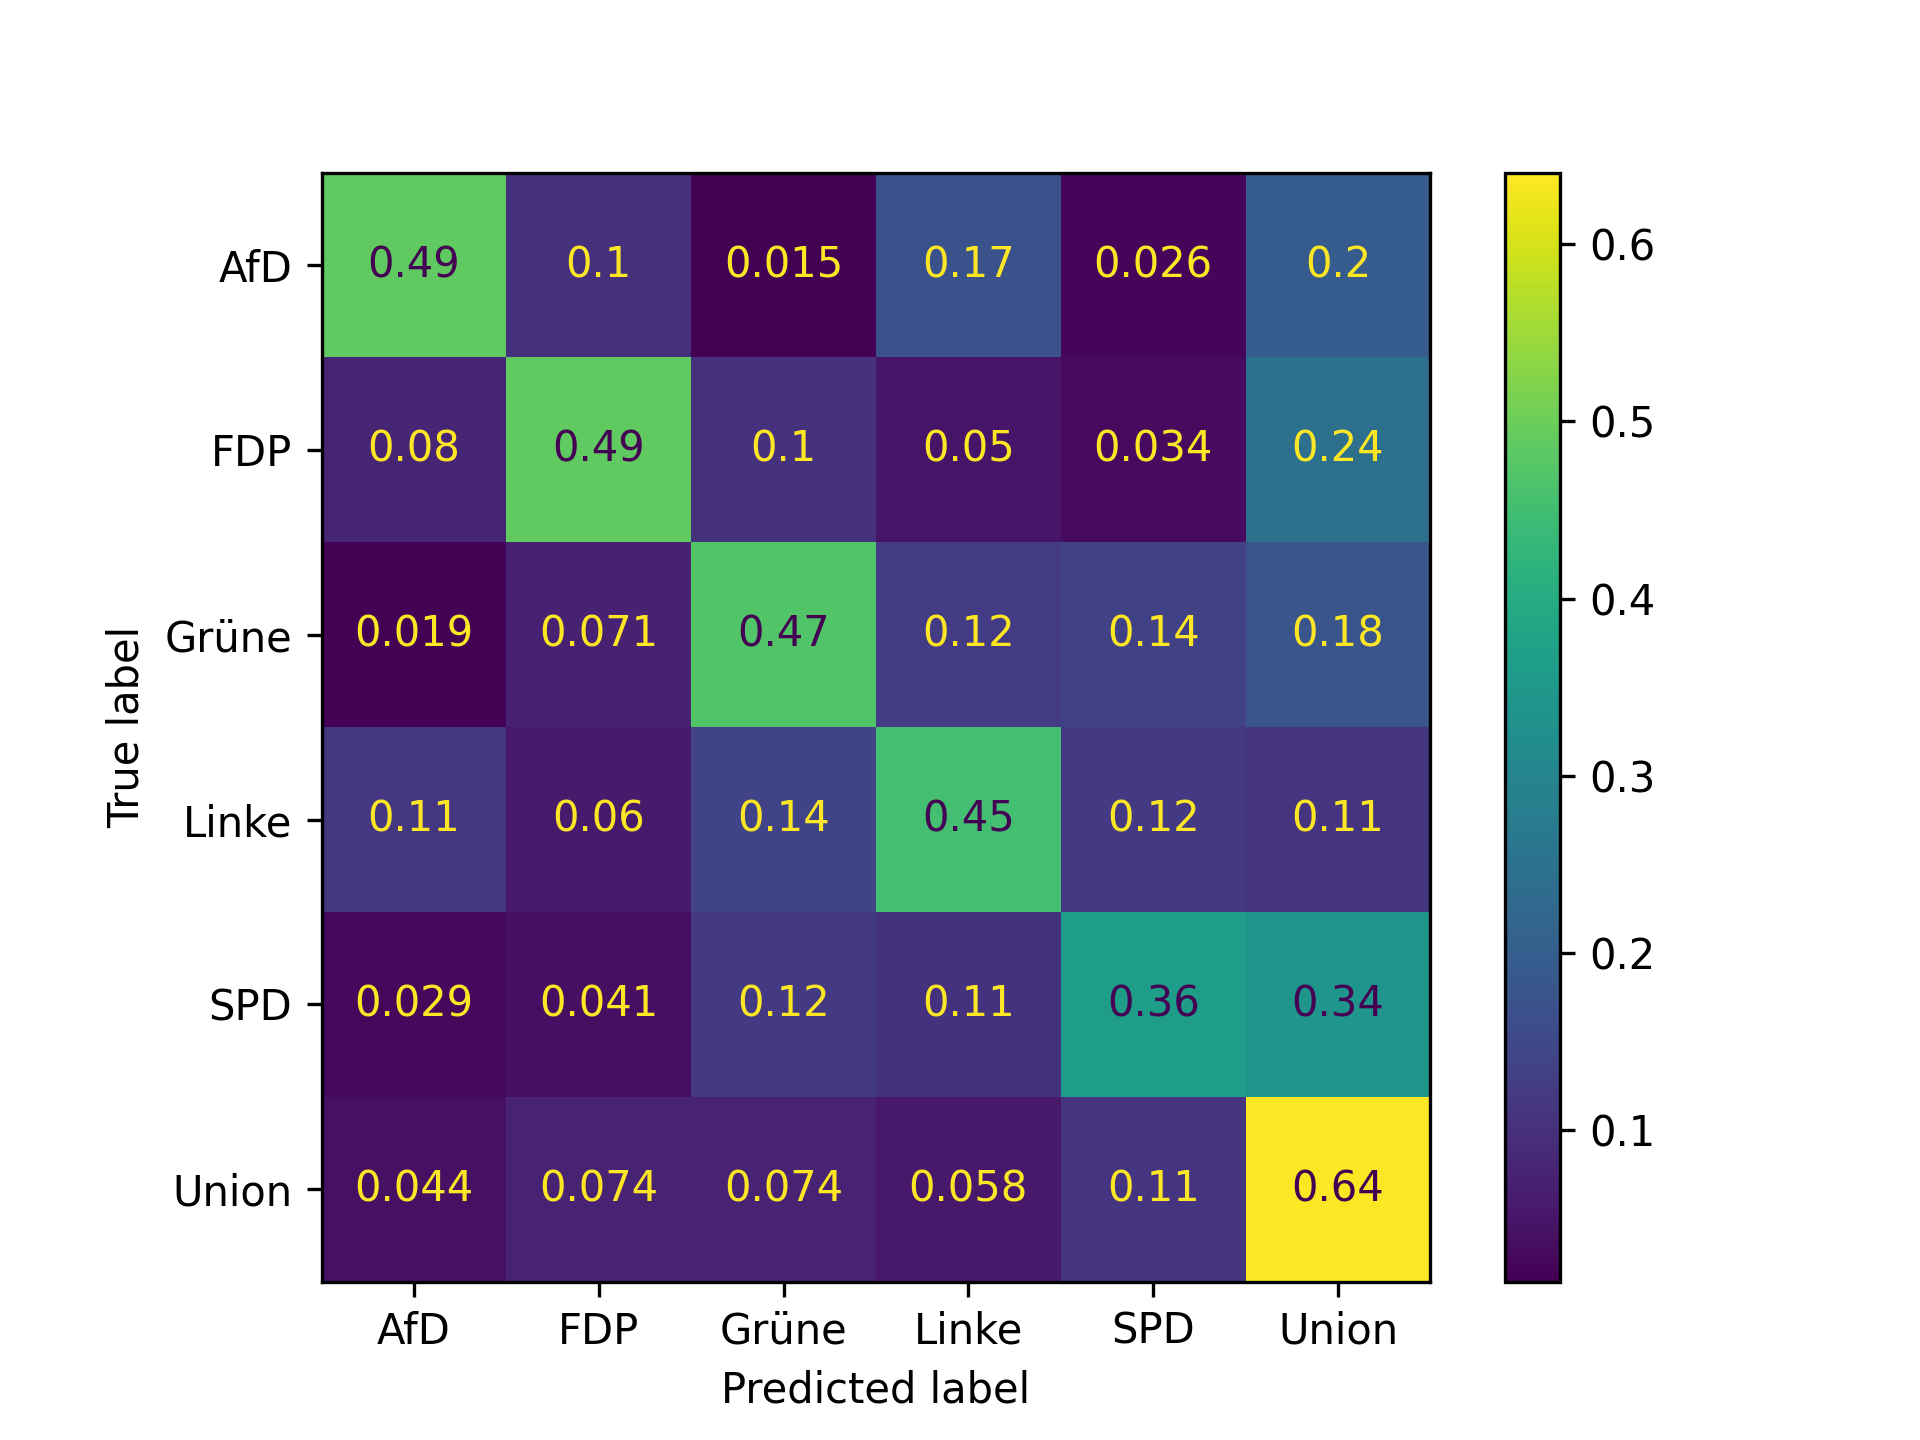
\includegraphics[width=\textwidth]{data/images/modeling/cnn/none/party_programs_confusion_matrix.png}
        \caption{Wahlprogramme}
        \label{sfig:confusionMatrixCnnManifestUnbalanced}
    \end{subfigure}
    \hfill
    \begin{subfigure}{0.49\textwidth}
        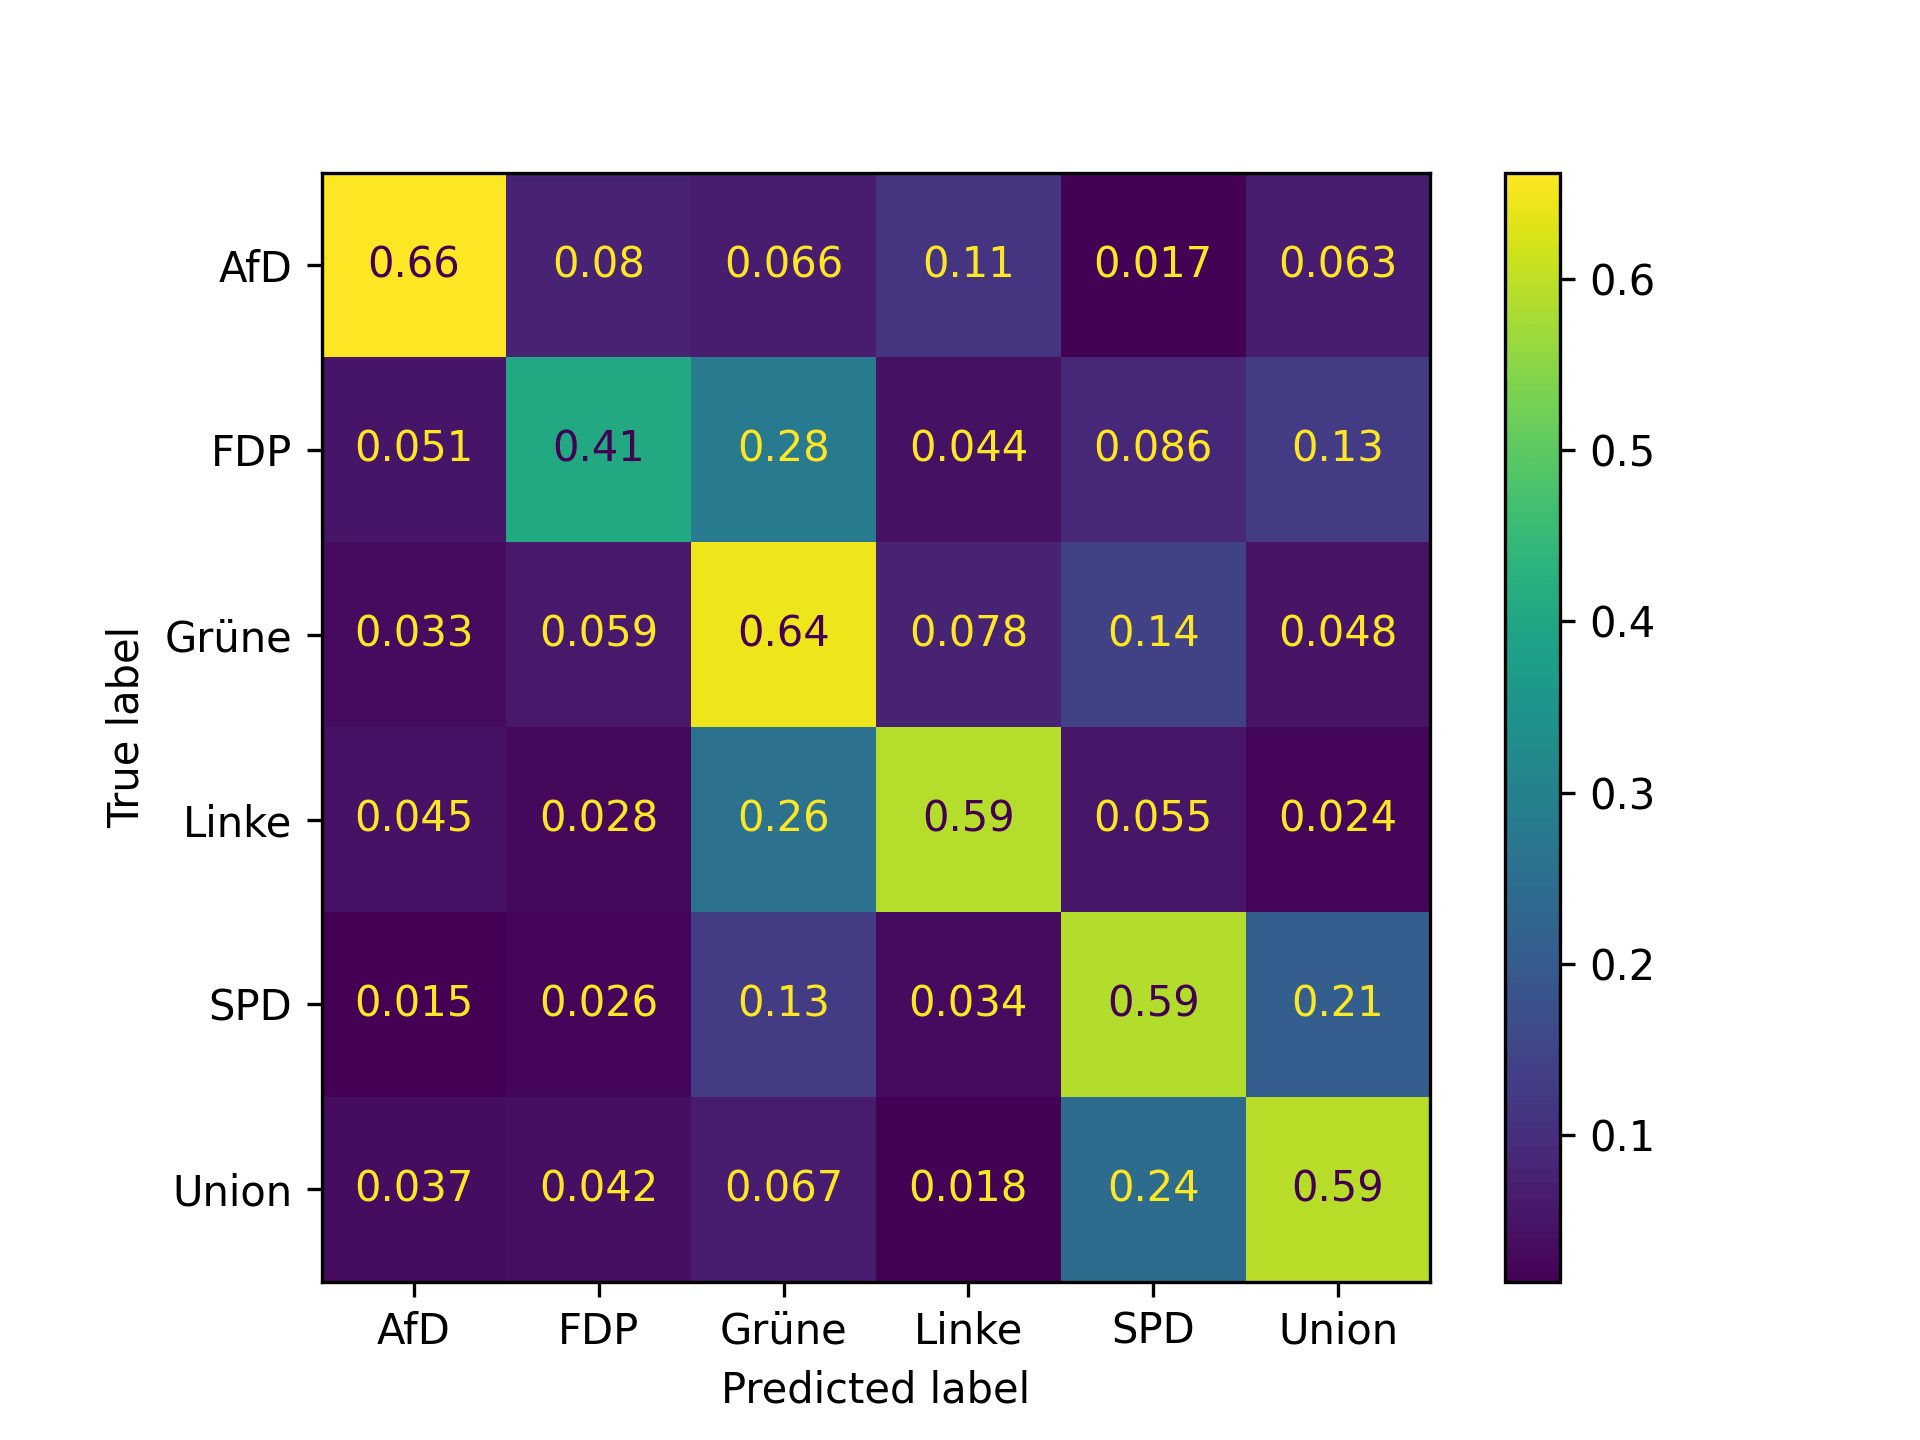
\includegraphics[width=\textwidth]{data/images/modeling/cnn/none/speeches_confusion_matrix.png}
        \caption{Reden}
        \label{sfig:confusionMatrixCnnSpeechesUnbalanced}
    \end{subfigure}
    \hfill
    \begin{subfigure}{0.49\textwidth}
        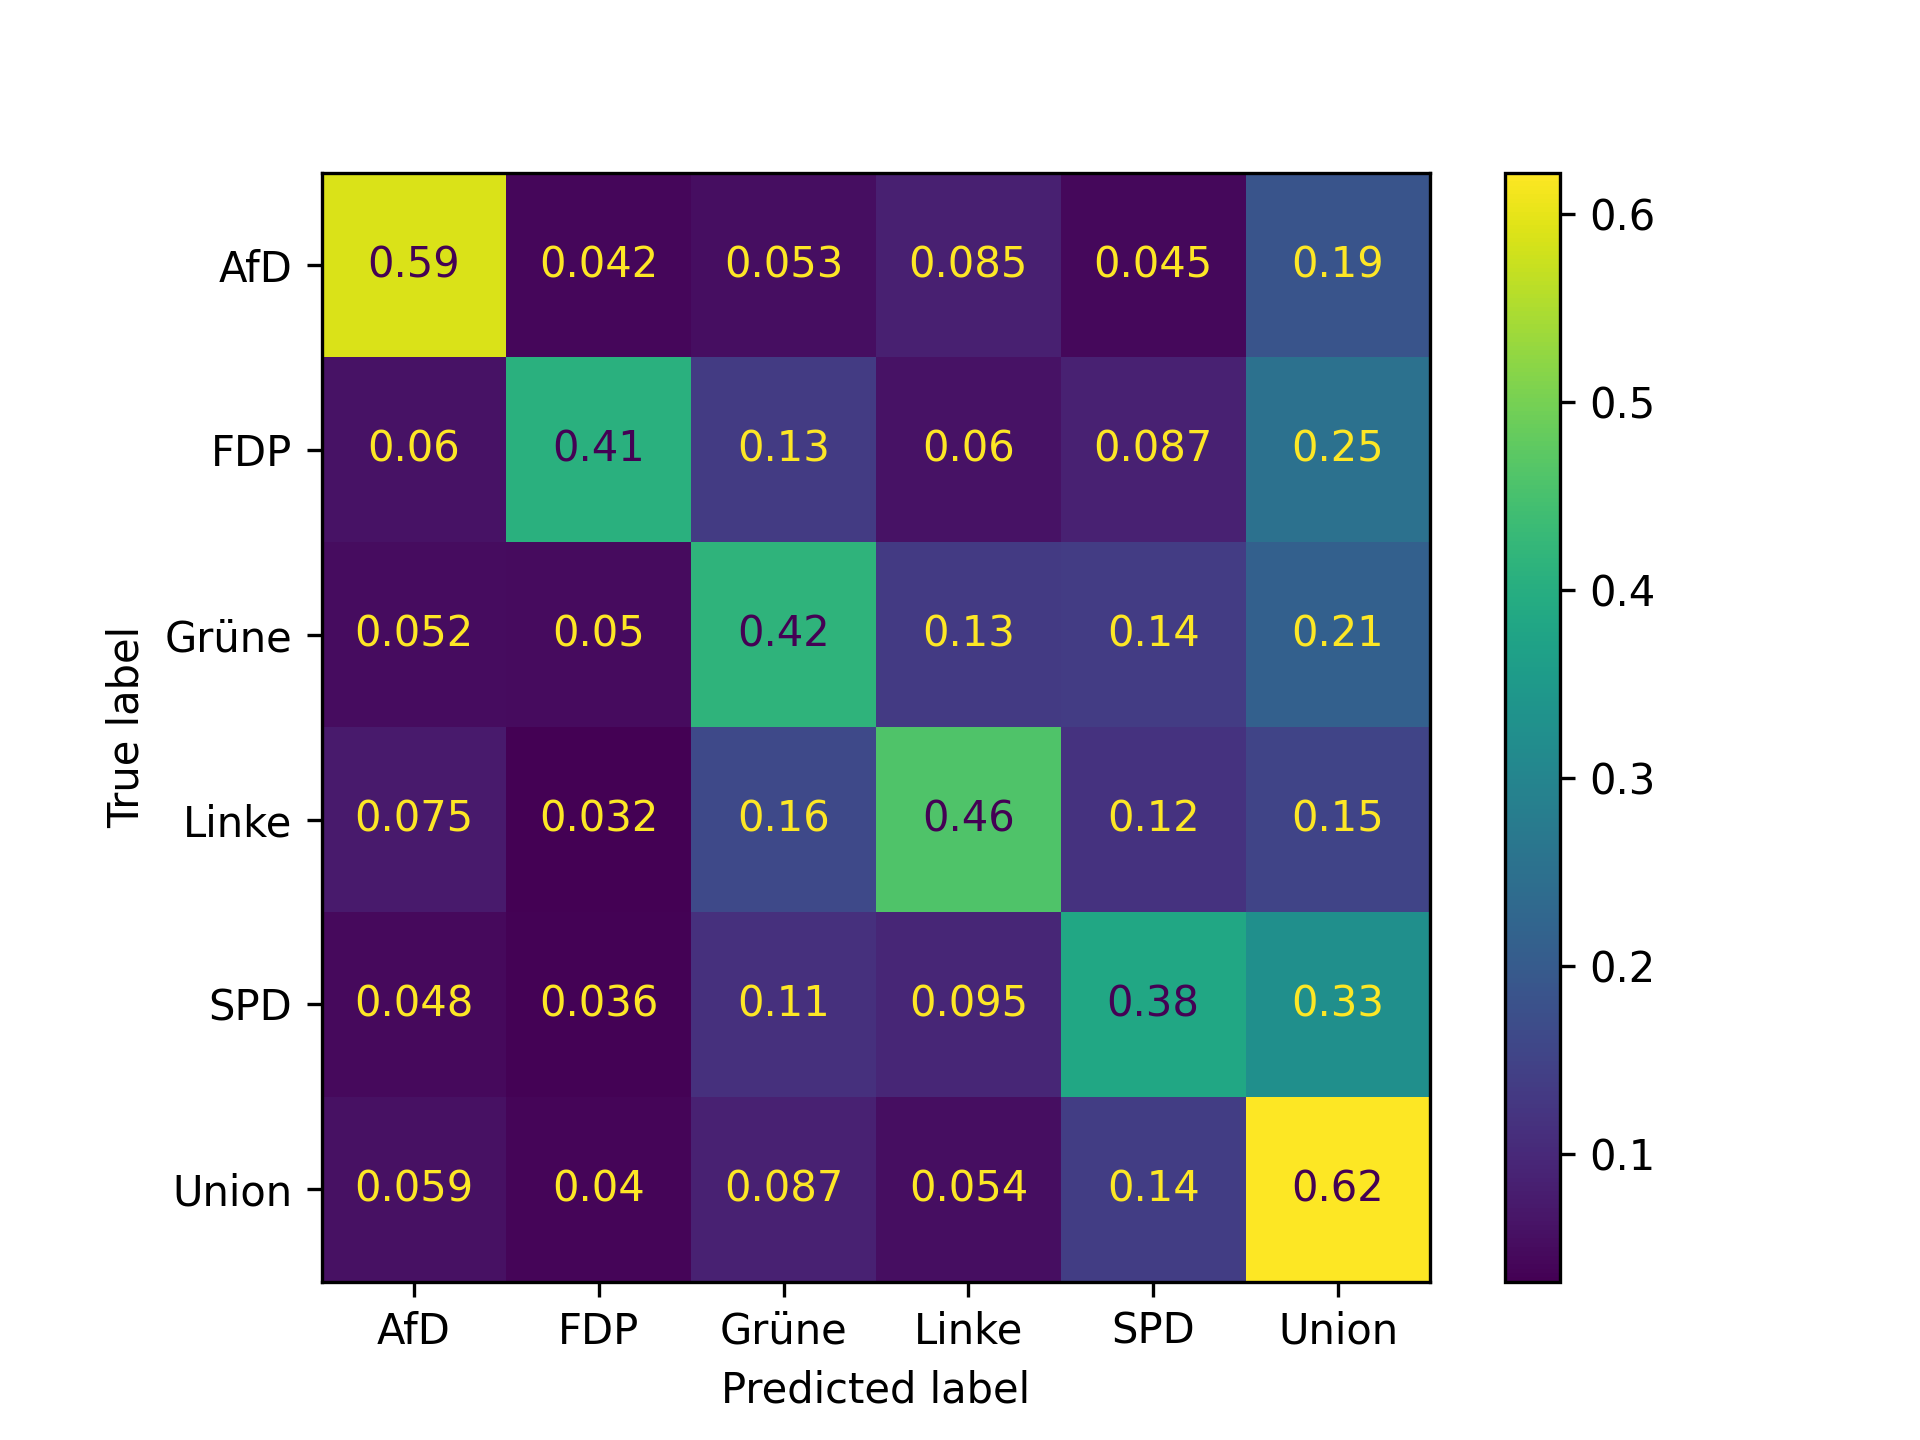
\includegraphics[width=\textwidth]{data/images/modeling/cnn/none/all_confusion_matrix.png}
        \caption{Kombiniert}
        \label{sfig:confusionMatrixCnnAllUnbalanced}
    \end{subfigure}
    \caption{Konfusionsmatrizen für das \acs{CNN}-Modell auf unausgeglichenen Datensätzen} \label{fig:confusionMatrixCnnUnbalanced}
\end{figure}

\subsection*{BERT}

\begin{figure}[H]
    \centering
    \begin{subfigure}{0.49\textwidth}
        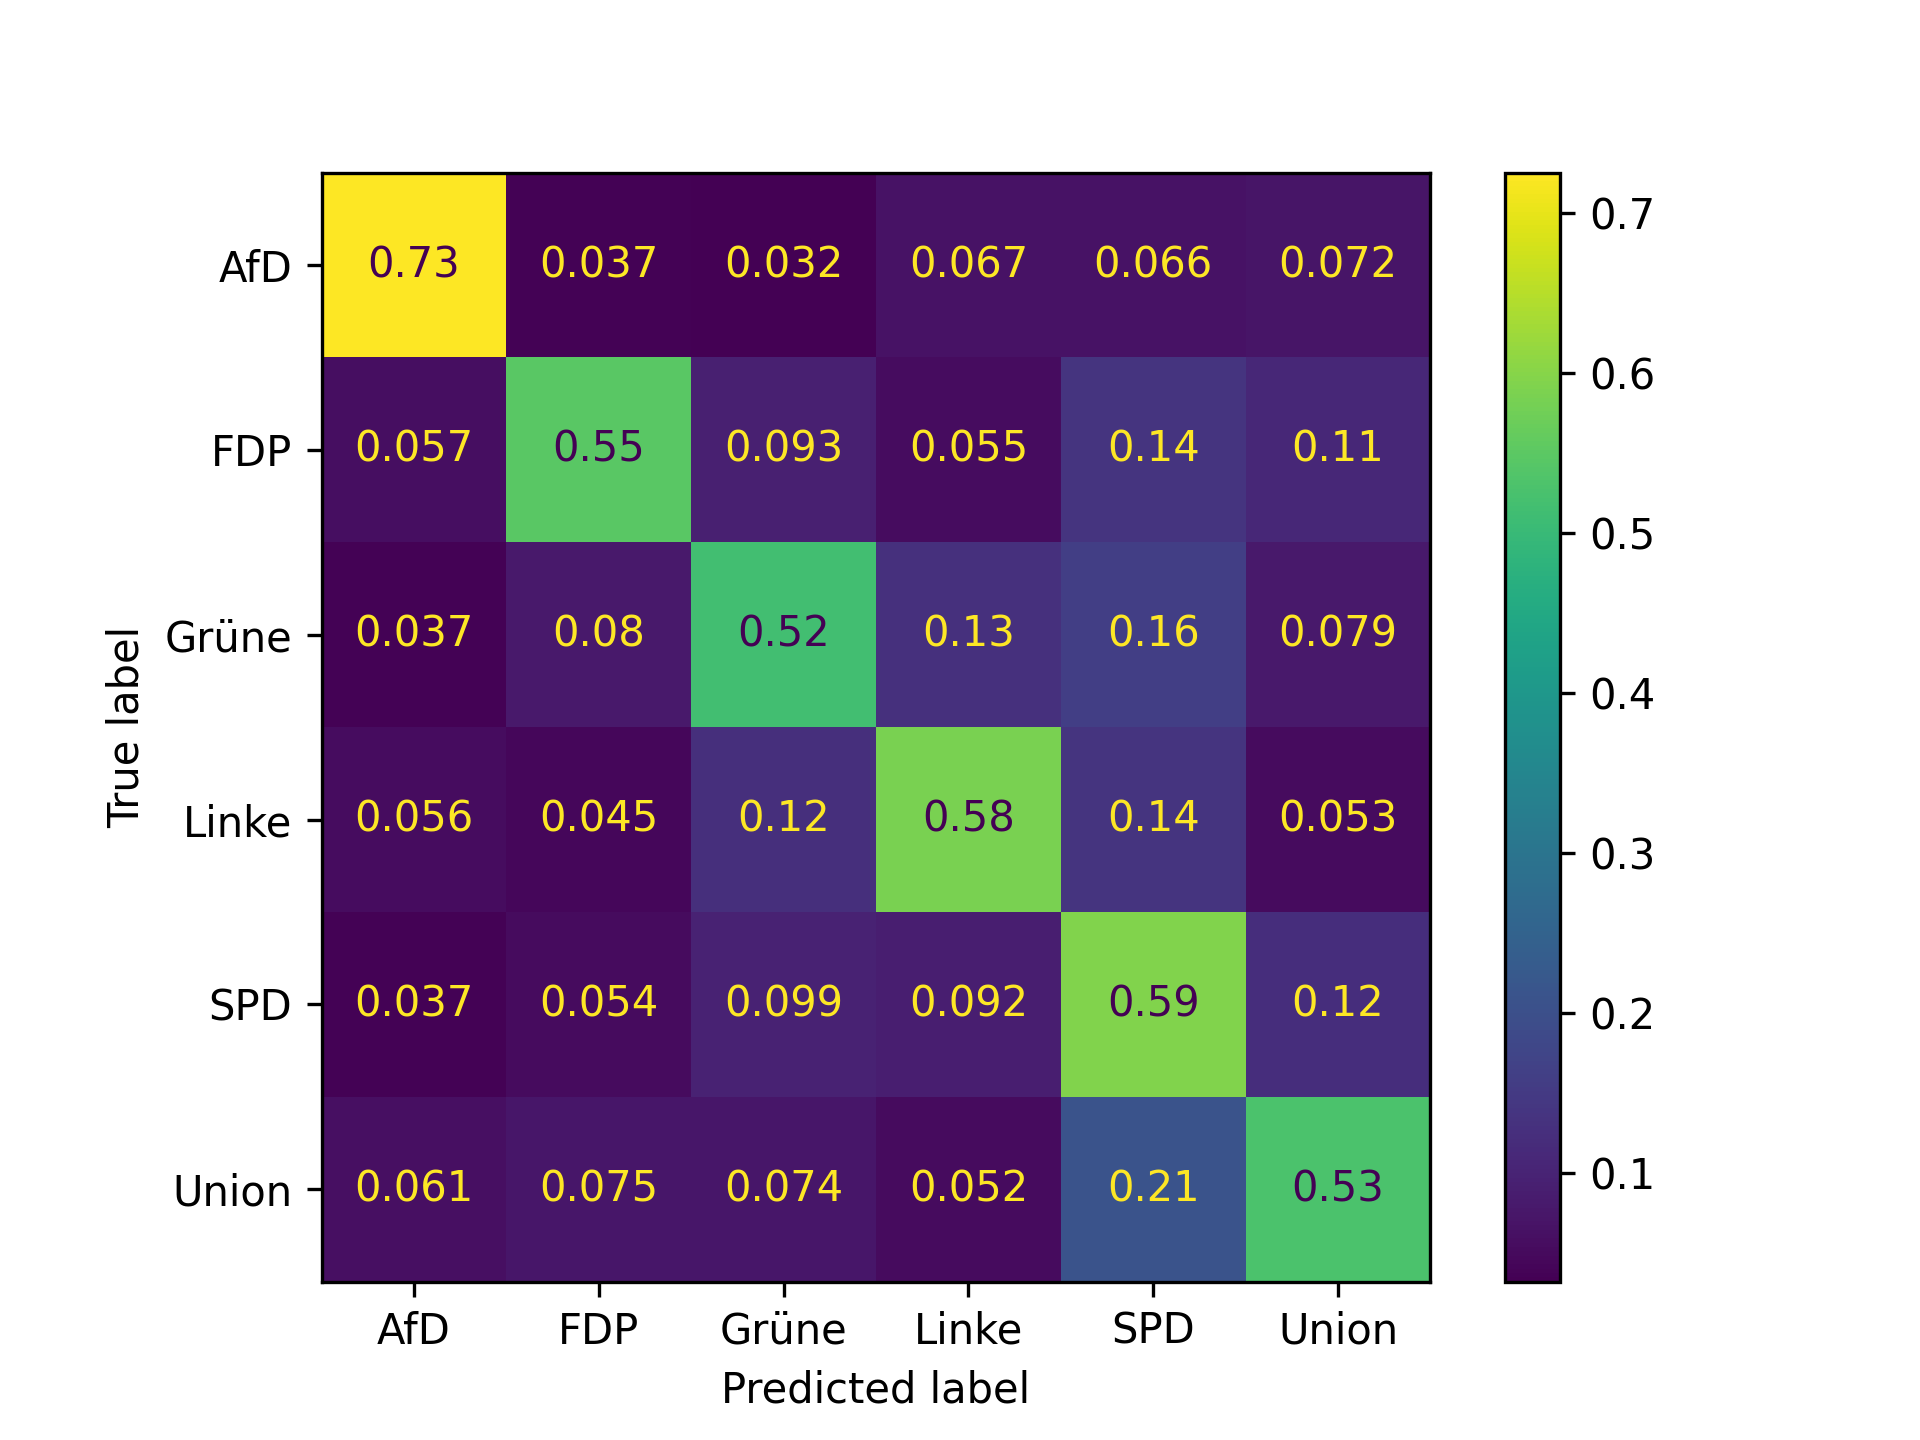
\includegraphics[width=\textwidth]{data/images/modeling/bert/none/tweets_confusion_matrix.png}
        \caption{Tweets} \label{sfig:confusionMatrixBertTweetsUnbalanced}
    \end{subfigure}
    \hfill
    \begin{subfigure}{0.49\textwidth}
        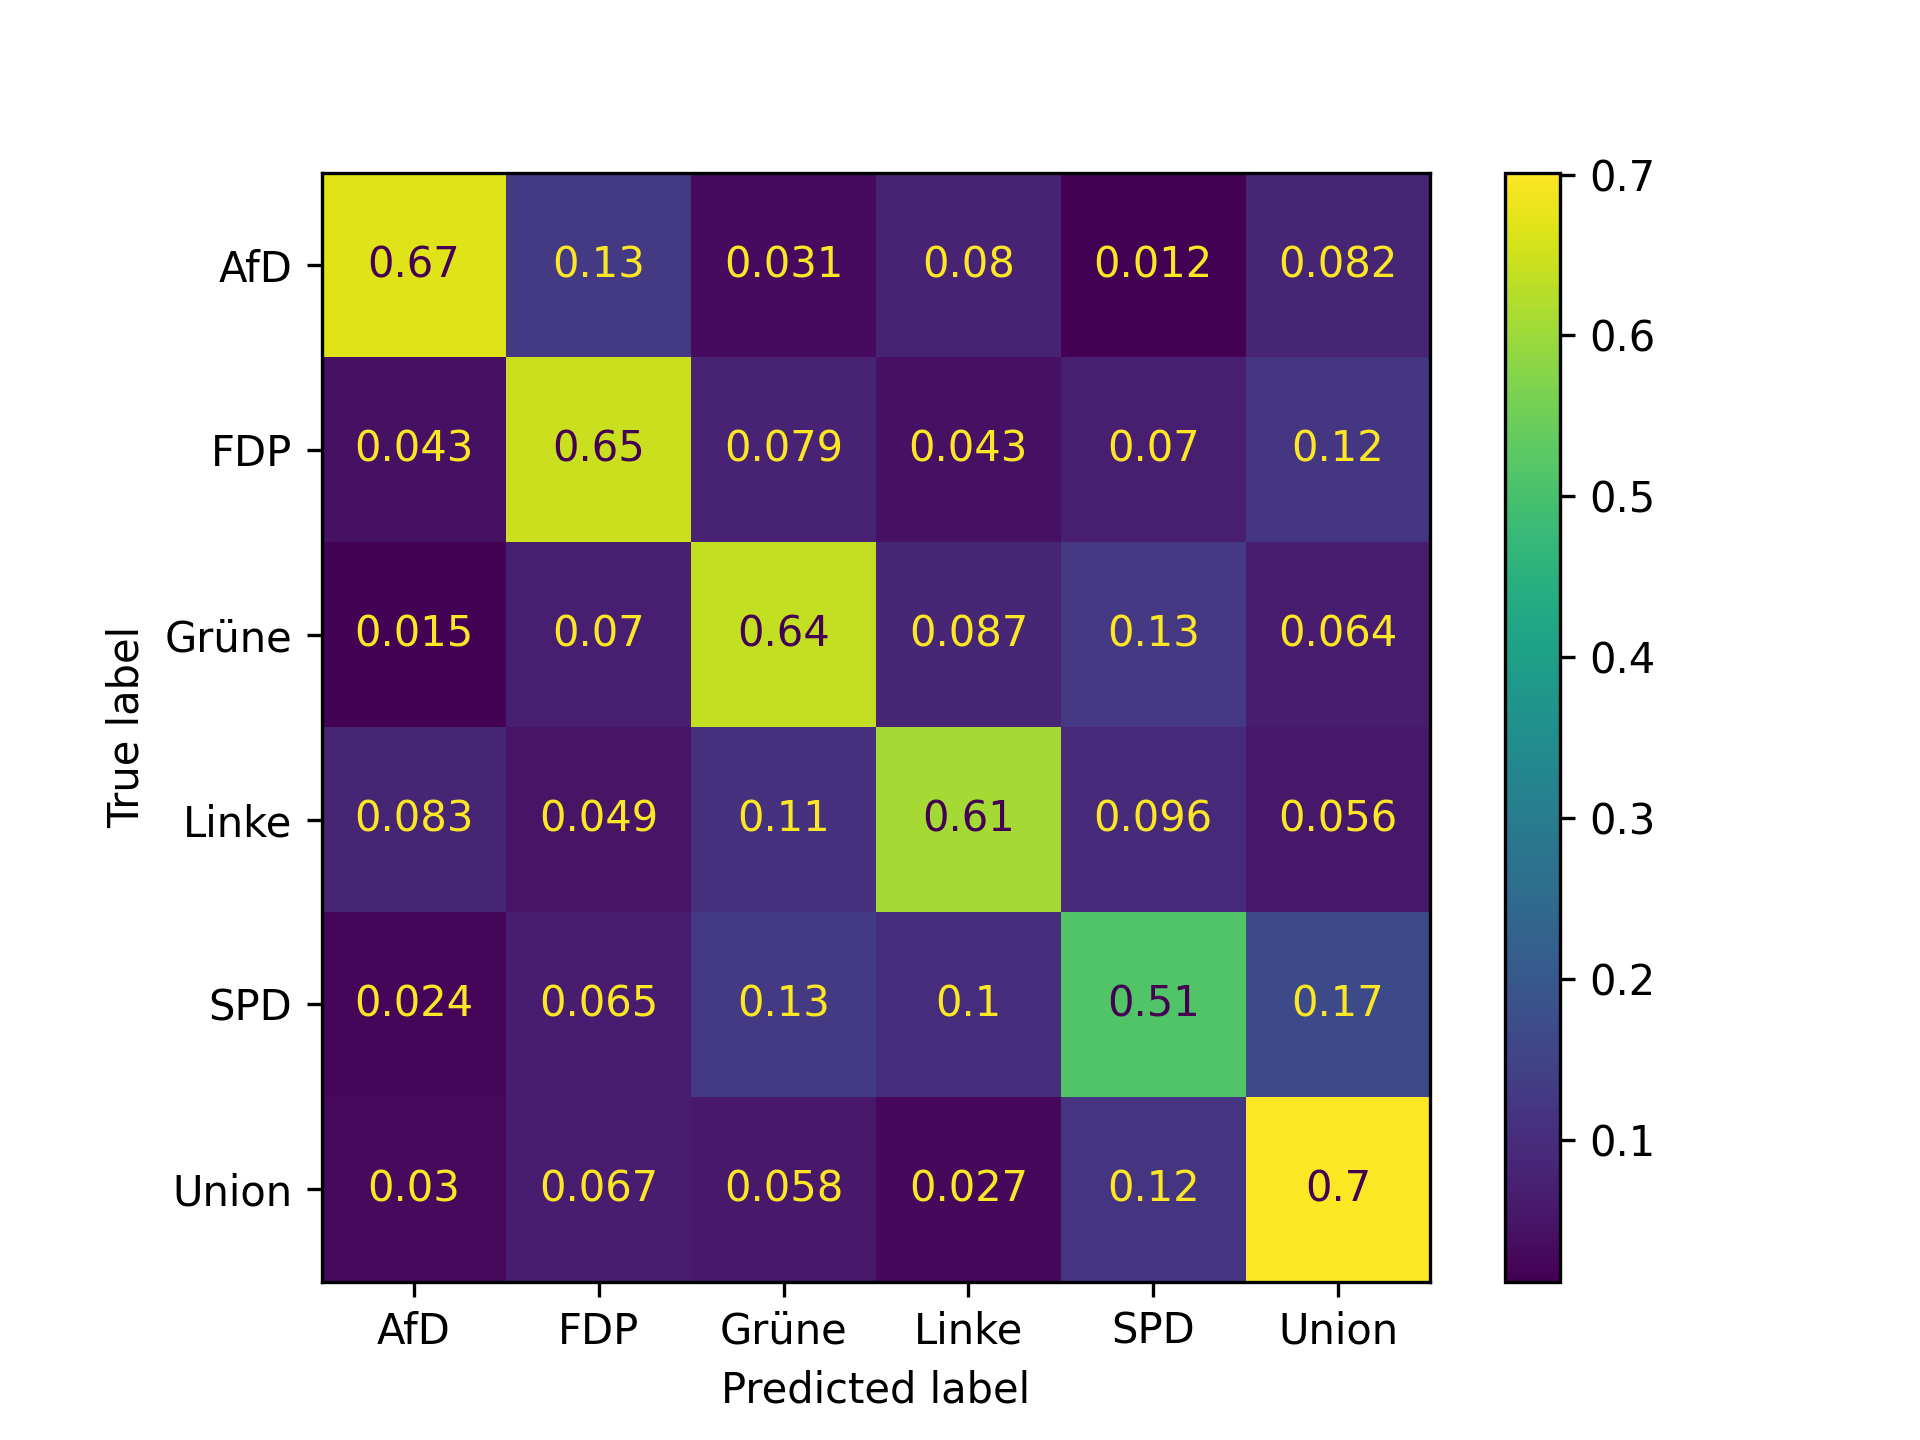
\includegraphics[width=\textwidth]{data/images/modeling/bert/none/party_programs_confusion_matrix.png}
        \caption{Wahlprogramme} \label{sfig:confusionMatrixBertManifestUnbalanced}
    \end{subfigure}
    \hfill
    \begin{subfigure}{0.49\textwidth}
        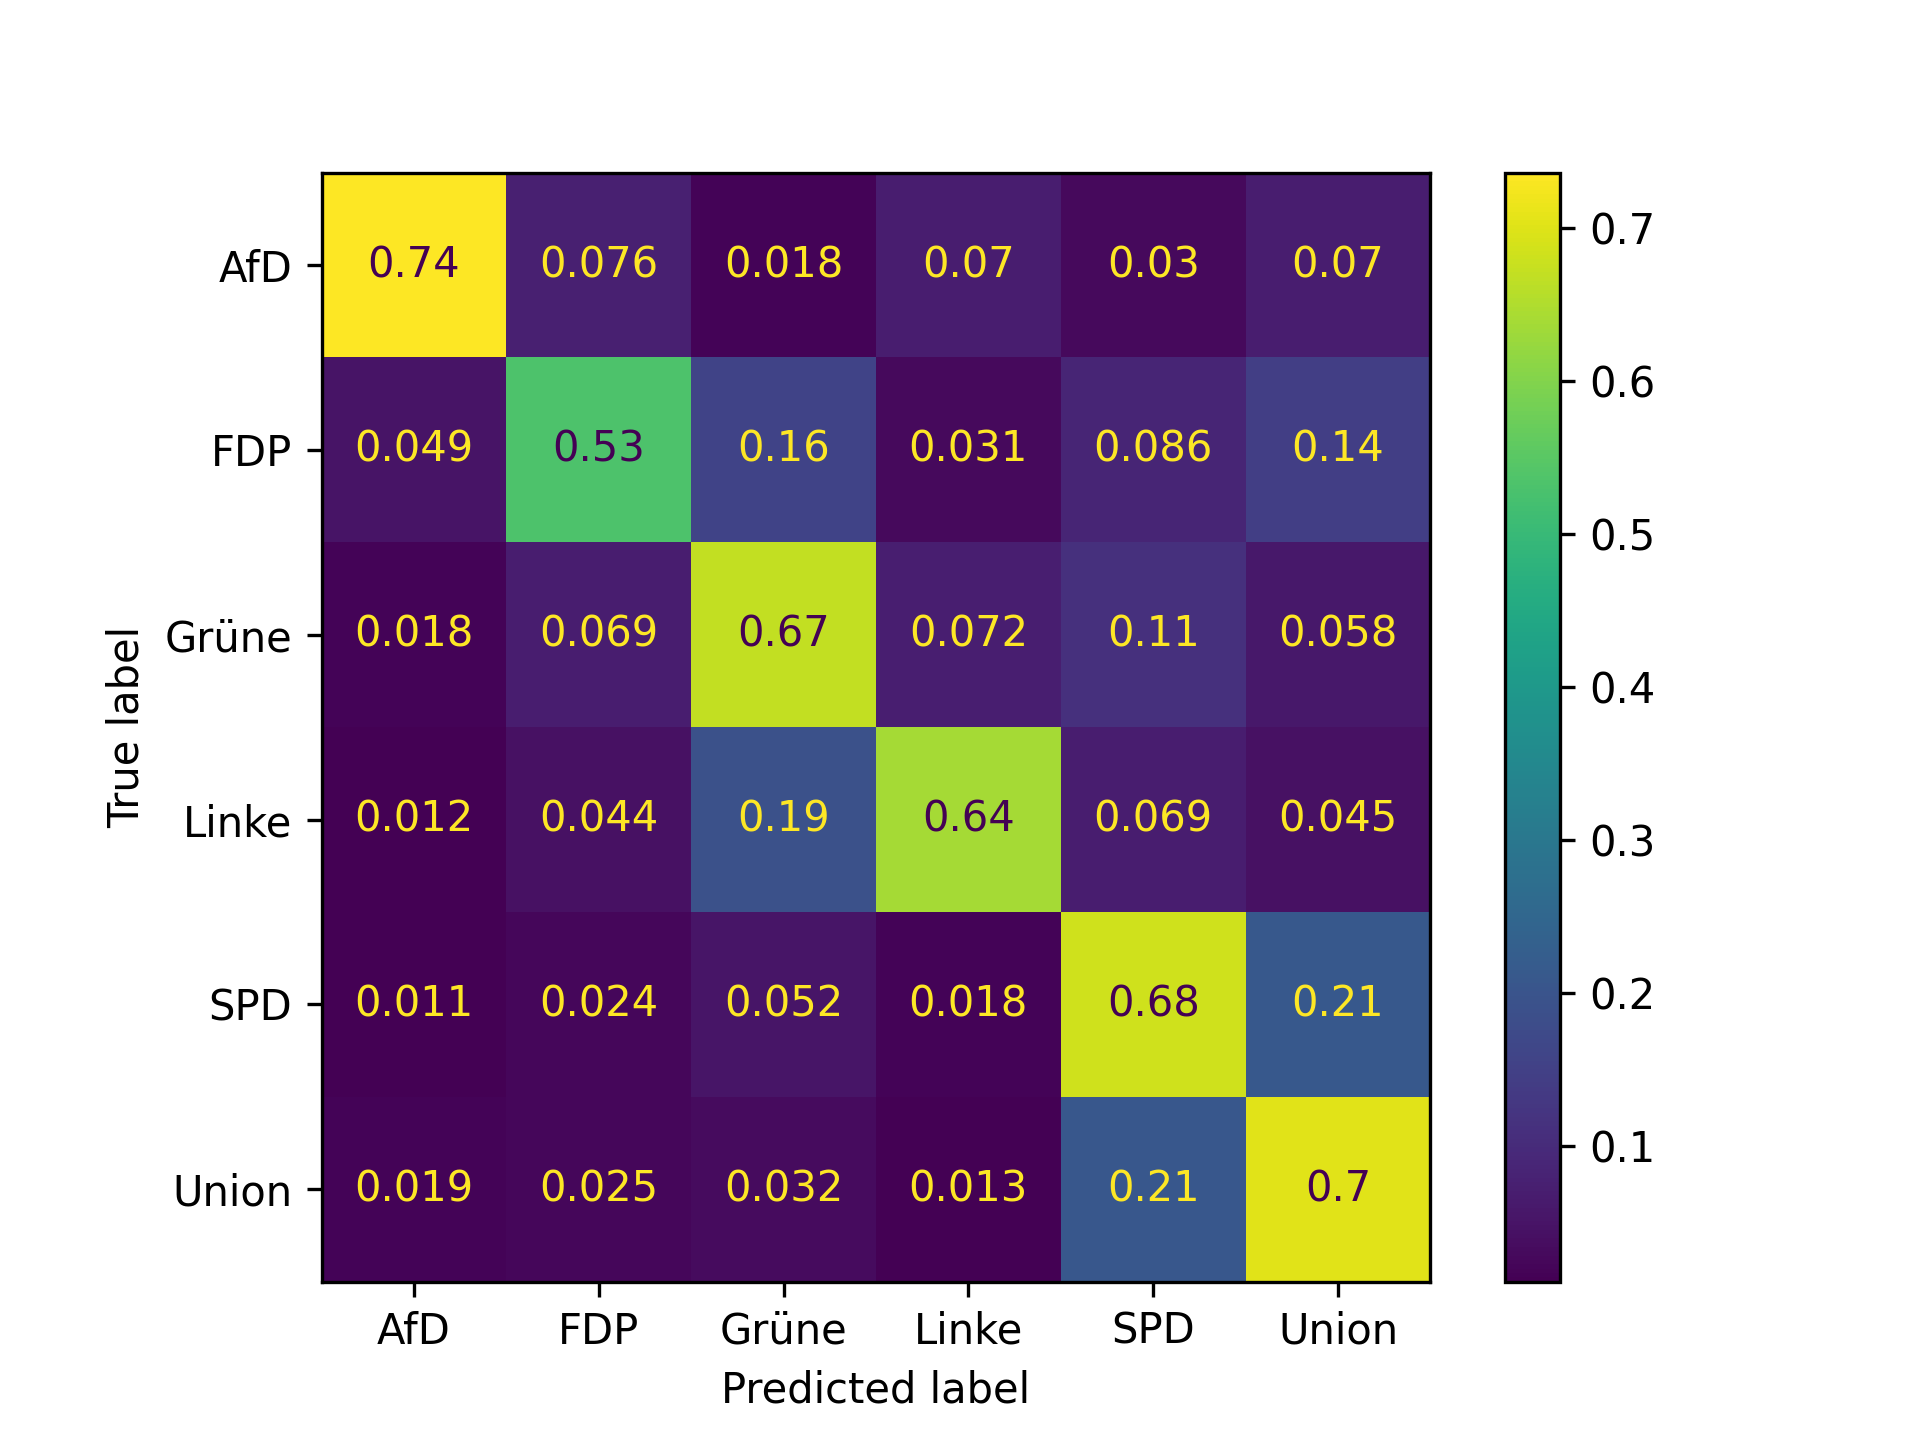
\includegraphics[width=\textwidth]{data/images/modeling/bert/none/speeches_confusion_matrix.png}
        \caption{Reden} \label{sfig:confusionMatrixBertSpeechesUnbalanced}
    \end{subfigure}
    \hfill
    \begin{subfigure}{0.49\textwidth}
        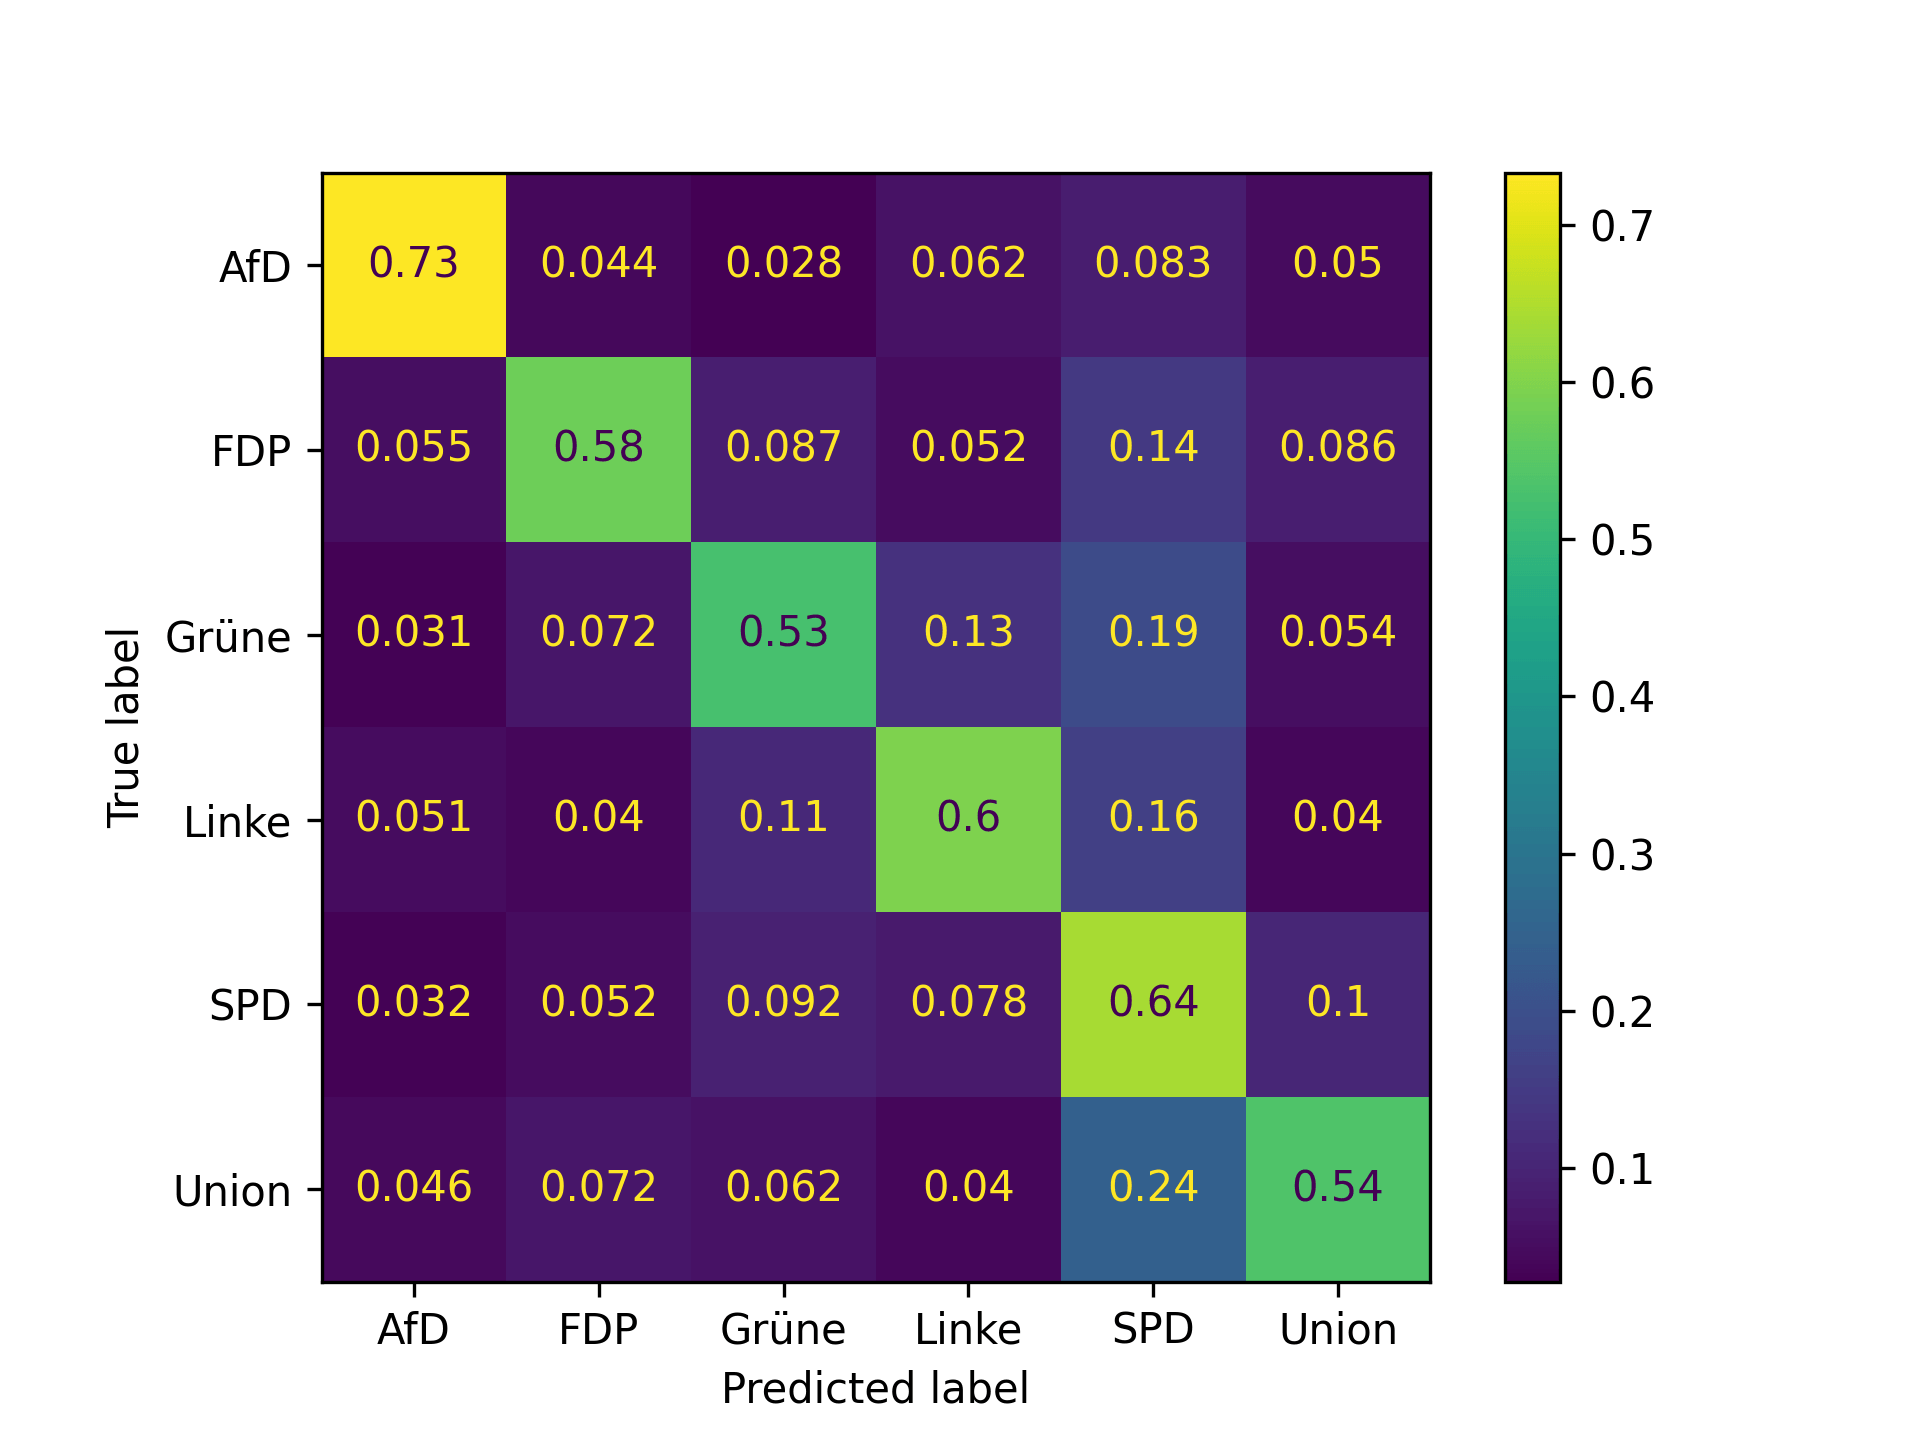
\includegraphics[width=\textwidth]{data/images/modeling/bert/none/all_confusion_matrix.png}
        \caption{Kombiniert} \label{sfig:confusionMatrixBertAllUnbalanced}
    \end{subfigure}
    \caption{Konfusionsmatrizen für DistilBERT auf unausgegelichenen Datensätzen} \label{fig:confusionMatrixDistilbertUnbalanced}
\end{figure}
